\chapter{Formaliser connaissances et hypothèses, vers un modèle de simulation co-construit : SimFeodal}
\label{chap:chap2}
\begin{center}
	{\large Version 2018-06-07\\
		(Incorporation brute du chapitre Peupler la Terre +\\ Ajout commentaires manuels +\\ Ajout schémas)}
\end{center}
\minitoc

\clearpage
\subsection*{Code couleur}
\begin{itemize}
	\item Texte publié dans le chapitre de Peupler la Terre
	\item {\blueroman Texte ajouté}
	\item {\redroman Texte publié dans le chapitre à supprimer (pour comparaison)}
\end{itemize}


\begin{mdframed}[backgroundcolor=gray!10,footnoteinside=false]
{\blueroman
	\textbf{Avertissement au lecteur}\\

Ce chapitre constitue en large partie une reprise d'un chapitre d'ouvrage, rédigé collectivement, intitulé \citetitle{cura_transition_2017} \autocite{cura_transition_2017}.
Le chapitre présenté ici est une version individuelle, fortement retravaillée et amendée, et contenant en particulier de nombreuses illustrations inédites.

Si le présent chapitre est un travail individuel, il présente toutefois un modèle collectif, dont l'auteur ne peut donc revendiquer l'unique paternité.
Les co-concepteurs de ce modèle sont les auteurs du chapitre sus-mentionné, c'est-à-dire :
\begin{itemize}
	\item Cécile Tannier, géographe, Directrice de Recherche, CNRS
	\\UMR Chrono-Environnement -- Besançon ;
	\item Samuel Leturcq, historien, Maître de Conférence, Université François Rabelais
	\\UMR CITERES-LAT -- Tours ; 
	\item Elisabeth Zadora-Rio, archéologue, Directrice de Recherche émérite, CNRS
	\\UMR CITERES-LAT -- Tours ;
	\item Élisabeth Lorans, archéologue, Professeure, Université François-Rabelais \\
	UMR CITERES-LAT -- Tours;
	\item Xavier Rodier, archéologue, Ingénieur de Recherche HDR, CNRS 
	\\UMR CITERES-LAT -- Tours ;
\end{itemize}
}
\end{mdframed}

\section{Introduction}

La question de l'émergence de la société féodale en Occident est au cœur d'un débat historique ancien.
Depuis le XVIIIe siècle, les penseurs cherchent à comprendre le fonctionnement de la société médiévale et à cerner ses fondements.
Les archives sont continûment explorées pour comprendre isolément et précisément les multiples facteurs à l'œuvre dans les processus qui ont fait émerger une société dite « féodale » dans le courant des Xe-XIe siècles.
Cette compréhension se heurte toutefois à la très grande complexité de ces processus, qui peuvent varier chronologiquement, mais aussi présenter des nuances infinies en fonction des zones étudiées.
Ces difficultés sont encore amplifiées par l'accès aux données, très variable selon l'état de la documentation, soumise aux aléas de la conservation ; d'une manière générale, les historiens des temps féodaux travaillent sur des documents rares et lacunaires, vestiges d'une société fondamentalement portée par l'oralité.

Depuis une quarantaine d'années, l'afflux massif de données de fouilles issues du développement de l'archéologie préventive a permis de renouveler et enrichir ces débats.
Les sources textuelles, qui apportent un éclairage plutôt normatif de la société, peuvent désormais être confrontées à des sources matérielles propres à mieux cerner les dimensions pratiques.
Toutefois, cette complémentarité des approches textuelles et matérielles, loin de simplifier les questionnements portant sur la société féodale, les a encore complexifiés en mettant en évidence des aspects anthropologiques et des différenciations géographiques jusqu'alors sous-estimés.
Le débat s'en est trouvé vivifié, se focalisant désormais sur la question de l'occupation de l'espace, considéré comme un marqueur efficace des transformations sociales.
L'émiettement et la dissémination des pouvoirs, dont témoigne la multiplication des châteaux (seigneuries châtelaines), se font concomitamment à l'apparition d'un réseau très structuré d'encadrement religieux (paroissialisation de la société), tandis que se fixe de manière définitive un système de peuplement fondé sur un maillage villageois, cœur d'une vie communautaire active.

C'est donc autour de l'articulation de ces trois éléments fondamentaux de la société féodale (châteaux, églises paroissiales, villages) que portent aujourd'hui analyses et théories.
Fixation, polarisation et hiérarchisation des centres de peuplement sont désormais les grands processus sociaux examinés à la loupe pour aborder la société médiévale.
Les historiens médiévistes analysent l'« encellulement » de la société \autocite{fossier_enfance_1982}, pistant d'une part les rôles polarisateurs du château (phénomène d'\textit{incastellamento} \autocite{toubert_les_1973}) et de l'église paroissiale accompagnée de son cimetière, considérés comme points de ralliement des populations paysannes, et d'autre part les manières dont les populations organisent collectivement les espaces de production (terroir villageois) pour assurer une répartition équilibrée des ressources.

Dans ce contexte, la période 800-1100 est habituellement considérée comme une période de transition, durant laquelle la société féodale se structure, certains évoquant la « révolution de l'an Mil »\autocite{fossier_enfance_1982}, tandis que d'autres tempèrent en parlant de « révélation de l'an Mil » \autocite{barthelemy_societe_1993}(« révélation » par l'augmentation en quantité et en qualité de la documentation textuelle).
Les hypothèses sont ainsi nombreuses, et il est difficile de trancher en faveur de l'une ou l'autre, tant l'articulation des facteurs sociaux, politiques, institutionnels, économiques et culturels est complexe.

Dans le cadre de l'ANR TransMonDyn, l'objectif, pour la transition des années 800-1100, est d'étudier les processus à l'œuvre dans la dynamique de fixation, polarisation et hiérarchisation de l'habitat rural.
L'approche est résolument géographique ; ce sont les implications spatiales des changements sociaux qui sont au cœur de l'étude.
La modélisation ne porte pas sur les transformations politiques et sociales elles-mêmes, mais sur leur impact sur le système de peuplement.
Le cœur du questionnement réside dans l'examen de la combinaison des facteurs ayant permis, entre 800 et 1100, la formation d'agrégats de foyers paysans dans une forme hiérarchisée et durable, polarisés par des châteaux ou des églises.
Il s'agit d'analyser, par la modélisation et la simulation informatique, les conditions d'émergence du maillage villageois.

\subsection{Délimitation temporelle de la transition}

\subsubsection{Régime 1}

Le régime R1 correspond à une situation observable au moment de l'essor carolingien
Vers 800, l'expansion territoriale franque s'achève, avec un empire couvrant la plus grande partie de l'Europe, de l'Èbre (Catalogne) à l'Elbe (confins slaves)
Le pouvoir est centralisé : le souverain s'assure de la fidélité des grands aristocrates en leur distribuant des terres réparties à travers tout l'empire, des charges politiques, ainsi que des richesses (or, argent, esclaves...) acquises au cours des raids annuels contre les peuples païens confinant les territoires francs

En 800, le système de peuplement régional est composé d'un semis de petits villages (consistant en un rassemblement assez lâche de quelques habitations) et d'unités d'exploitation isolées
Ces villages et unités d'exploitation sont peu pérennes et se caractérisent par des changements de localisation au bout d'un siècle ou deux à des distances allant de quelques dizaines à quelques centaines de mètres
Les villes qui existent en l'an 800 sont des chefs-lieux de cité hérités de l'Antiquité
Elles ont une fonction centrale en tant que siège épiscopal, mais leur rôle sur le plan économique et administratif est relativement peu important.

\subsubsection{Régime 2}
On fixe le régime R2 aux alentours de 1100, à une époque où l'autorité royale est en déclin, et où le territoire sur lequel elle se manifeste concrètement s'est réduit à une échelle provinciale.
La réalité du pouvoir politique est aux mains de dynasties comtales accaparant les prérogatives de la puissance publique (justice, service militaire, fiscalité).
Les rois n'interviennent pratiquement plus dans les domaines de leurs grands vassaux qui ont eux-mêmes constitué leurs propres réseaux de fidèles.
Ces lignages aristocratiques ne peuvent plus accroître leur pouvoir qu'en spoliant leurs voisins : ces rivalités entraînent une forte militarisation de la société.
Les coûts induits par celle-ci (construction de châteaux, frais d'armement, entretien de chevaliers...) font que les seigneurs exercent une forte pression fiscale sur les paysans.
En raison de l'affirmation du pouvoir ecclésiastique, l'encadrement religieux de la société laïque est très fort.
Les villes existant en 800 se sont développées : de nouveaux noyaux d'habitat ont émergé autour de monastères suburbains, qui concurrencent la cité épiscopale et développent des activités de production et d'échange.
L'armature urbaine est en outre renforcée par l'émergence de petites villes, souvent associées à des prieurés et des bourgs monastiques ayant chacun leurs enceintes.
Cette configuration spatiale du peuplement correspondant au régime 2 s'est maintenue jusqu'à la Révolution française et même après, les prémices de hiérarchie dans le système de peuplement mis en place s'intensifiant jusqu'à cet événement.


\subsection{Transformations entre 800 et 1100}

Au cours de la transition, des changements notables se produisent à différents échelons spatiaux.

\subsubsection{Au niveau de l'ensemble de l'Europe du Nord-Ouest}

Sous l'effet de différents facteurs d'ordre surtout conjoncturel (crises de succession, pression exercée par les raids vikings mais aussi sarrasins, fin de l'expansion territoriale de la Chrétienté...), l'empire se fragmente de façon répétée, d'abord en royaumes, puis en principautés.
Le modèle économique carolingien, principalement fondé sur la conquête militaire et une économie de razzia (tributs, esclaves), se transforme.
Le tarissement de cette source de revenus entraîne un affaiblissement des récompenses que pouvait donner l'autorité centrale.


\subsubsection{Au sein des sous-ensembles régionaux (provinces, principautés)}

En réaction à la perte de pouvoir de l'autorité centrale, la compétition pour la terre et les ressources augmente, attisant un climat de violence et d'affrontements générateur de structures défensives et d'une recherche de protection.
On assiste ainsi à l'apparition des premiers châteaux forts, qui se multiplient et maillent l'espace étudié.
Dans le même temps, l'encadrement religieux des populations se renforce au niveau local avec la création d'un réseau paroissial, organisé selon un semis de centres ecclésiaux constitués chacun d'une église paroissiale et de son cimetière.
Les droits attachés aux églises, de nature fiscale (la dîme) ou religieuse (obligation d'assister aux offices dominicaux, de recevoir les sacrements et d'être inhumé dans le cimetière attenant), déterminent la formation des territoires paroissiaux.
Ce faisant, l'Europe se couvre de son « blanc manteau d'églises » selon l'expression fameuse de Raoul Glaber au début du XIe siècle.
Le coût de ces nouveaux édifices et de l'entretien du clergé chargé de les animer est amorti par des dons de plus en plus importants de la part des seigneurs laïcs (sous forme matérielle – prieurés, terres – et immatérielle – droits d'usages, droits de basse justice), et par une ponction croissante sur les  paroissiens (dîmes en particulier).
Le clergé parvient ainsi à polariser, autour des églises paroissiales, des fidèles qui lui apportent contrôle social et revenus.
Ces changements politiques et sociaux ont un fort impact sur le système de peuplement.
On assiste à la mise en place d'un nouveau maillage territorial (paroissial et seigneurial), et à une polarisation de l'habitat autour des lieux de pouvoir (églises, châteaux), entraînant l'émergence de nouveaux chefs-lieux.
Ces phénomènes de polarisation, plus ou moins importants selon les attracteurs, aboutissent à une hiérarchisation du système de peuplement, entre petites villes, villages et hameaux.
Cette polarisation est renforcée par une structuration communautaire de la société paysanne.
Ces communautés agraires (ou rurales), fondées sur un principe de solidarité, organisent non seulement l'exploitation du territoire nourricier, particulièrement des res.
sources pacagères, mais aussi leur rapport avec les seigneurs.
Les paysans y trouvent un intérêt économique par la rationalisation des pratiques agricoles (par exemple assolement, gestion des pacages communs...), mais aussi un contrepoids dans les rapports de force qui les opposent à leurs souverains laïcs ou ecclésiastiques.

\subsection{Aire d'étude}	

La modélisation du mouvement général de fixation et polarisation de l'habitat entre 800 et 1160 \footnote{
	Cette date a été choisie afin que le modèle dépasse, en termes d’emprise temporelle, la durée de la transition à proprement parler, et ainsi vérifier que les dynamiques simulées s’inscrivent dans la durée.
} suppose de représenter les effets polarisants des églises paroissiales et des châteaux.
Pour ce faire, il convient de travailler à une échelle montrant la construction du maillage paroissial et castral entre 800 et 1160, c'est-à-dire une zone assez vaste, de l'ordre d'un diocèse par exemple.
La zone historique de référence à partir de laquelle s'est engagée l'expérience de modélisation est la Touraine, soit le cadre de l'ancien diocèse de Tours ; ce choix a été guidé par une connaissance historique particulière.
ment poussée des dynamiques de peuplement pour la période 800-1160, et de l'existence d'indicateurs quantitatifs pouvant servir à étalonner correctement les modèles \autocite{zadora-rio_paroisses_2008}.

\section{Premières étapes de modélisation}

\subsection{Identification des entités impliquées dans la transition}\marginnote{\hl{Développer !}}[-30pt]

La première étape de la modélisation de cette transition a été d'identifier et de décrire les entités spatiales impliquées dans celle-ci.
Ce travail s'est appuyé sur une grille de lecture géographique qui permet d'observer un système de peuplement selon trois niveaux d'analyse qui sont dans le cas de la transition 800-1100 :
\begin{itemize}
	\item Des entités spatiales élémentaires
	\begin{itemize}
		\item l'unité d'exploitation, qui comporte un centre d'exploitation (habitat et	annexes) ainsi que les terres qui en dépendent;
		\item le ressort seigneurial, qui est le territoire de l'exercice du pouvoir d'un	seigneur (une rivière, un moulin, un territoire plus ou moins vaste...) et peut comporter différentes parcelles, d'un seul tenant ou dispersées;
		\item le ressort paroissial, territoire sur lequel l'église exerce son action, qui est une entité spatiale émergente au cours de la transition.
	\end{itemize} 
	
	\item Des entités spatiales mésoscopiques
	\begin{itemize}
		\item 	les villages qui consistent en un rassemblement plus ou moins lâche d'unités d'exploitation. Ils peuvent être ou non un lieu de marché ou de foire et inclure ou non un château, une église ou un monastère;
		\item les villes qui comportent plusieurs paroisses, des cours seigneuriales, des marchands, des artisans et des paysans;
	\end{itemize}
	
	\item Une entité spatiale de niveau macroscopique, la région du nord-ouest de l'Europe chrétienne en 800.
\end{itemize}

Pour décrire les processus à l'œuvre au cours de la transition il est également nécessaire d'identifier des entités sociales actrices des changements qui
se déclinent en sept catégories :
\begin{itemize}
	\item les foyers paysans (familles) disposent d'une unité d'exploitation dans	laquelle ils exercent une polyactivité agricole;
	
	\item les foyers d'artisans-marchands vendent leur production artisanale sur les marchés ou les foires ; ils peuvent être localisés dans une ville ou dans un village;
	
	\item les foyers marchands, eux, ont la particularité d'être localisés uniquement dans les villes;
	
	\item les seigneurs laïques et leurs entourages (chevaliers etc.), chaque entité correspondant à une famille aristocratique, ses clients et son tribunal;
	
	\item les seigneurs ecclésiastiques, chaque entité correspondant à une communauté religieuse, ses clients (qui peuvent être des laïques) et son tribunal;		
	
	\item l'évêque, représentant du Saint-Siège à l'échelle du diocèse;
	
	\item enfin, l'autorité centrale (roi ou empereur).
\end{itemize}

Dans une publication antérieure, nous avons identifié et caractérisé les relations structurelles entre ces différentes entités spatiales et sociales \autocite[figure 13.1, p. 295]{tannier_ontologie_2014}.

\subsection{Identification des processus à l'œuvre dans la transition}

Afin de décrire le plus clairement possible les processus à l'œuvre au cours de la transition, nous avons choisi de multiplier les points de vue au moyen de	différentes représentations graphiques : diagrammes sagittaux et graphiques	processuels.
La figure 1 en est un exemple.
Elle décrit les actions effectuées par différentes entités sociales, représentées sous la forme de rectangles aux coins arrondis.
Ces actions entraînent la modification des attributs d'entités qui peuvent être soit sociales, soit spatiales (représentées sur la figure sous la forme de rectangles simples).
Ces modifications entraînent elles-mêmes (directement ou indirectement) une transformation de la configuration spatiale du peuplement : apparition d'églises, de prieurés et de châteaux ; changement de localisation des foyers paysans.

%	\subsection{Établissement de règles de comportement pour chaque entité sociale}
%	
%	L'établissement de règles de comportement des entités sociales consiste en l'identification de faits stylisés représentant certains aspects de la transition étudiée.
%	Le tableau 1 les décrit en mettant en correspondance les objectifs de chaque entité sociale avec les actions qu'elle peut entreprendre pour les atteindre.
%	Parmi ces actions, certaines influencent directement la configuration spatiale du système de peuplement : création de châteaux, de prieurés, de paroisses ; déplacement des foyers paysans.
%	D'autres actions permettent d'accroître le pouvoir des entités concernées, et donc l'attractivité des sièges de pouvoir (châteaux, prieurés, abbayes) ou bien des villages quand ils possèdent une communauté agraire (ou rurale) puissante.
%	Ces actions ont une implication spatiale indirecte.
%	
%	\begin{figure}[!h]
%		\centering
%		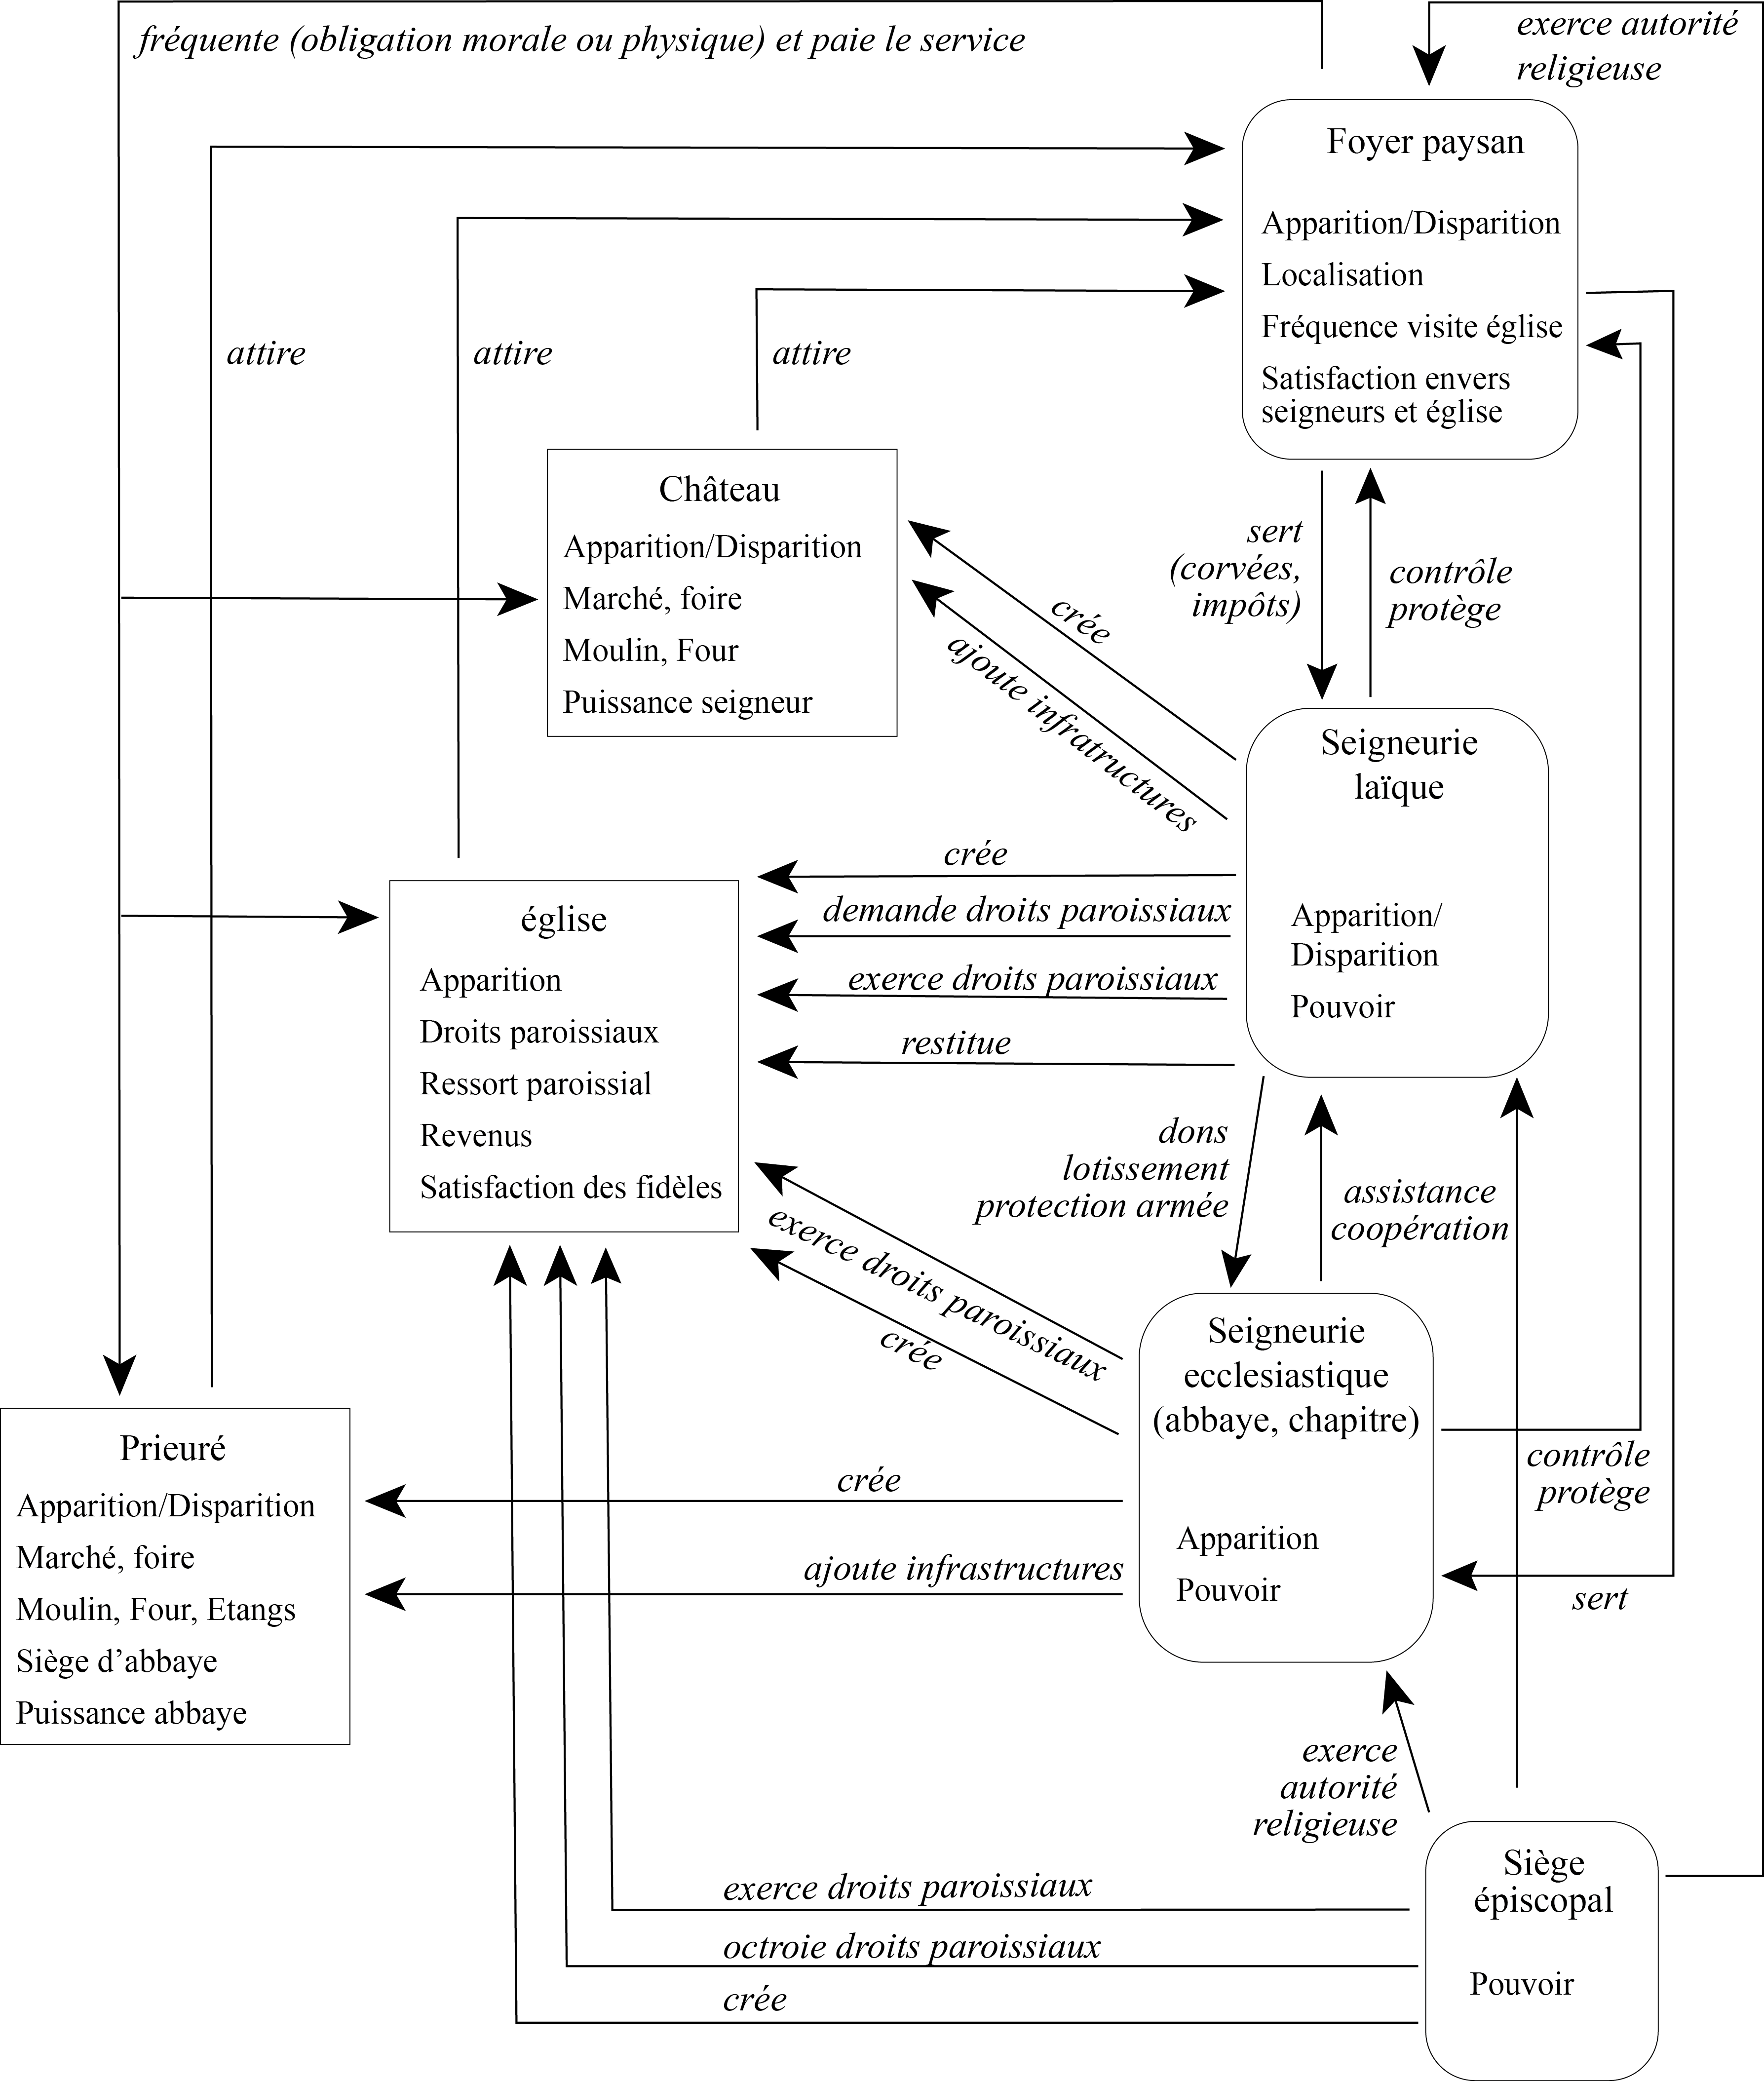
\includegraphics[width=1\linewidth]{src/Chapitre_TMD/Fig1}
%		\caption{Actions de différentes entités sociales et spatiales ayant un impact direct ou indirect sur la configuration spatiale du peuplement régional de l’Europe du Nord-Ouest entre 800 et 1100.}
%		\label{fig:fig1}
%	\end{figure}
%	
%	
%	D'autres entités avaient été identifiées lors des premières étapes de modélisation comme ayant un rôle majeur dans la transition.
%	Le choix a été fait d'écarter celles qui n'avaient pas d'influence spatiale directe (monde marchand) ou pas de représentation spatiale à une échelle régionale (c'est le cas notamment de l'autorité centrale [roi ou empereur] et du Saint-Siège).
%	
\begin{figure}[H]
	\centering
	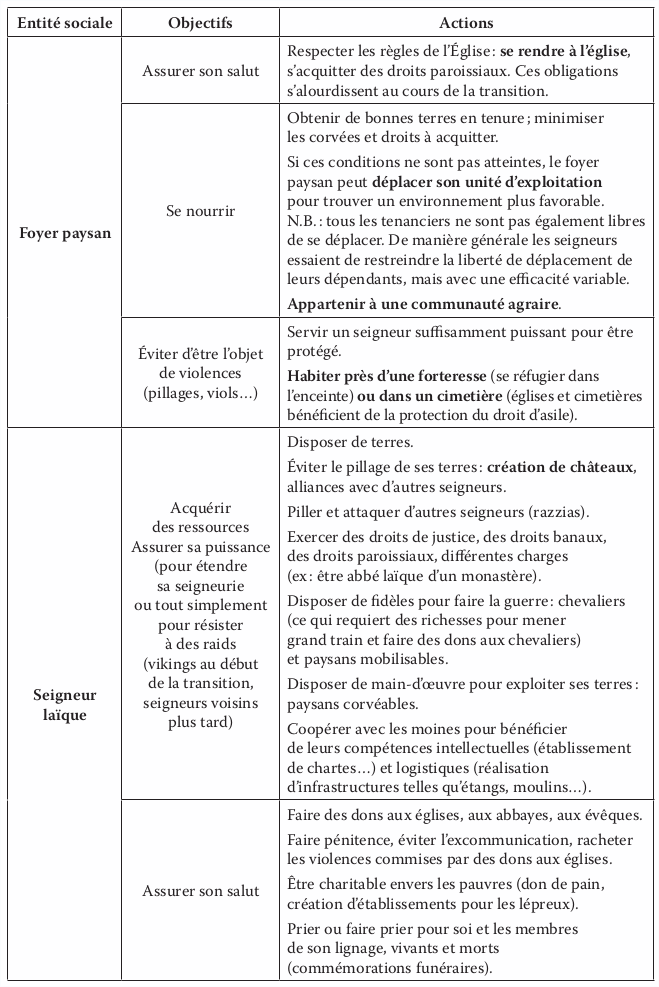
\includegraphics[width=1\linewidth]{src/Chapitre_TMD/Tab1_1.png}
\end{figure}

\begin{figure}[H]
\centering
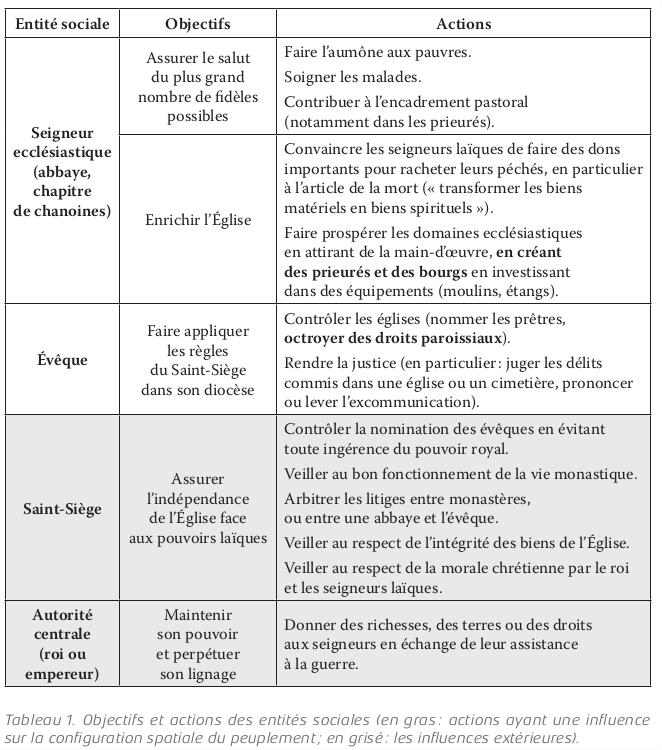
\includegraphics[width=1\linewidth]{src/Chapitre_TMD/Tab1_2.png}
\marginnote{\hl{Supprimer les trois dernières lignes (eveque, saint-siege et autorité centrale du tableau)}}[-50pt]
\end{figure}

\subsection{Vers un modèle de simulation multi-agents de la transition : SimFeodal}

À l'issue de ce cheminement méthodologique et conceptuel, il a été possible de représenter une partie des processus à l'œuvre sous la forme d'un modèle de simulation.
L'objectif de ce modèle n'était pas de simuler les transformations politiques et sociales elles-mêmes, mais leur impact sur le système	de peuplement à un niveau d'analyse régional.
Les organisations régionales du peuplement sont très diverses en Europe du Nord-Ouest au cours de la période étudiée, mais elles présentent des traits communs que le modèle vise à reproduire.
Celui-ci doit donc être suffisamment générique pour s'adapter aux différents contextes régionaux via la modification, par l'utilisateur, des paramètres et des entrées du modèle sans toucher aux règles de comportement des agents.
Sur cette base, l'enjeu a été de trouver, au moyen d'une exploration par la simulation, les valeurs de variables et de paramètres permettant la reproduction des dynamiques observées en Touraine, le modèle et son paramétrage	devenant dès lors candidats à l'explication de ces dynamiques.

Le modèle doit être facile à comprendre et se prêter à la discussion, c'est pourquoi nous avons choisi d'adopter un formalisme multi-agents, dans lequel les comportements des entités modélisées sont représentés explicitement.
L'espace modélisé reproduit de manière stylisée les cadres d'une principauté de la période dite féodale.
Un pas de temps de simulation représente une durée de vingt ans.
La plate-forme de développement informatique choisie a été GAMA \autocite{grignard_gama_2013}.
Le modèle SimFeodal\footnote{
SimFeodal : \textbf{Sim}ulation de la \textbf{F}ixation, de l’\textbf{É}mergence et de l’\textbf{O}rganisation \textbf{D}ynamique d’\textbf{A}grégats de populations \textbf{L}ocalisés, URL : http://github.com/RCura/SimFeodal.
} est ici présenté et décrit dans sa version 4.4.

\section[Architecture générale]{SimFeodal : architecture générale du modèle multi-agents}

Comme la transition est étudiée sous l'angle des modifications spatiales qu'elle	produit, les agents du modèle sont soit spatiaux, soit socio-spatiaux.
De leurs interactions au cours d'une simulation doivent émerger les transformations du système de peuplement régional décrites précédemment.
Les agents représentés dans le modèle ont été définis sur la base des travaux menés sur la Touraine à partir des sources textuelles et archéologiques existantes pour la période \autocite{zadora-rio_paroisses_2008}.
Prospections et fouilles archéologiques livrent une riche base de données sur les dynamiques de l'occupation du sol pour la période 800-1160 (vestiges de fermes isolées, de hameaux, de villages, de sites castraux et monastiques...). 

Le matériau de base est donc par nature spatial.
Les sources textuelles, quant à elles, prennent la forme de sources narratives (chroniques, annales, histoires) et d'actes de la pratique (chartes et notices), qui font état d'événements, de transactions et de décisions pouvant affecter l'occupation du sol depuis le point de vue des puissants, seigneurs laïques et ecclésiastiques.
Le croisement des sources textuelles et matérielles enrichit la compréhension des comportements de chaque agent, mais aussi des interactions entre les agents.

\subsection{Les agents du modèle}

Les paysans, majoritaires dans la population, sont représentés au moyen d'agents « \textbf{Foyers paysans} » (tableau 2).
Les foyers paysans ont une représentation spatiale, correspondant à leur unité d'exploitation.
Il s'agit d'une abstraction, ne serait-ce que parce que les foyers paysans sont considérés comme persistants sur l'ensemble de la durée de la transition, s'approchant plus de la durée de vie du bâti que de celle de ses habitants.
Leur comportement dans le modèle représente uniquement les processus qui les poussent à modifier leur localisation.

\begin{figure}[H]
	\centering
	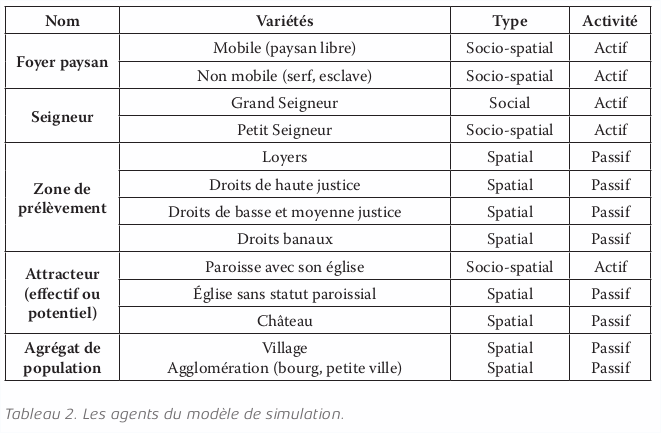
\includegraphics[width=1\linewidth]{src/Chapitre_TMD/Tab2.png}
	\marginnote{\hl{Modifier et développer tableau}}[-50pt]
\end{figure}

De la même manière et avec un niveau d'abstraction semblable, les puissants sont modélisés via des agents « \textbf{Seigneurs} ».
Ceux-ci traversent l'ensemble de la période, et tendent ainsi à être représentatifs des charges qu'ils détiennent plutôt que des individus à proprement parler, en particulier quand il s'agit de seigneurs ecclésiastiques.
Les petits seigneurs sont localisés dans l'espace modélisé et ont un rayon d'action limité autour de leur localisation tandis que les grands seigneurs ne sont pas localisés en un point de l'espace modélisé et peuvent intervenir en tous lieux.
Les actions des seigneurs correspondent à la création d'entités spatiales dépendant d'eux.
Il s'agit des « \textbf{Zones de prélèvement} », représentations spatiales des logiques de collecte de droits et redevances, et instruments de constitution de leur puissance.
Les zones de prélèvement sont de forme circulaire et de rayon très variable (de un à plusieurs kilomètres).
Les taux de prélèvement qui leur sont associés sont également variables. 
Quatre types de droits et redevances y sont collectés : loyers (terres exploitées), droits de haute justice (crimes de sang...), droits de basse et moyenne justice (contentieux...), droits banaux (utilisation des moulins, des fours...).
Les agents « attracteurs » créés par les seigneurs (« \textbf{églises} » et « \textbf{châteaux} ») sont des entités spatiales ponctuelles.
Quand les églises sont paroissiales, elles exercent une attraction sur les foyers paysans, ce qui fait d'elles des entités socio-spatiales.
Les agents « \textbf{Agrégats de population} » sont des entités spatiales génériques incluant villages et villes.
Chaque catégorie d'agents a des caractéristiques et des comportements
différents.
Les agents spatiaux sont localisés dans l'espace modélisé.
Les agents sociaux (ou socio-spatiaux) représentent des entités sociales sur le plan historique.
Les agents actifs se déplacent (c'est le cas des agents « foyers paysans »), ou bien créent ou modifient d'autres agents (les agents « seigneurs » peuvent créer des agents « châteaux » et « zones de prélèvement » ; les agents « églises paroissiales » peuvent modifier le contour des ressorts paroissiaux de leurs voisines).

\subsection{Dynamiques modélisées}

\begin{figure}[!h]
	\centering
	\includegraphics[width=1\linewidth]{src/Chapitre_TMD/Fig2}
	\caption{Les processus historiques observés en Touraine et leur introduction dans le modèle sous forme d’événements exogènes.}
	\label{fig:fig2}
\end{figure}

Dans le cadre de cette expérience de simulation, souhaitant analyser le libre jeu des agents soumis à des règles simples, nous avons repoussé tout \textit{deus ex machina} habituellement invoqué en guise de facteur explicatif des dynamiques observées.
Ainsi, nous ne postulons aucune hypothèse de crise ou de croissance économique (pas d'augmentation ou de diminution de la production, aucune prise en compte d'une éventuelle amélioration de la productivité ou des rendements).
Nous éliminons également l'hypothèse d'une croissance démographique.
Enfin, les dynamiques environnementales telles que, par exemple, l'optimum climatique, n'ont pas été prises en compte.
L'émergence d'un climat de violence interne à la région modélisée (figure 2), résultant de la conflictualité croissante entre seigneurs au cours du Xe siècle, est représentée dans le modèle par l'apparition puis l'augmentation d'un besoin de protection pour les foyers paysans.
Ceux-ci cherchent alors à se localiser aussi près que possible d'un château pour bénéficier de sa protection.
L'augmentation des obligations religieuses, résultant notamment du renforcement de l'encadrement ecclésiastique, se traduit, elle, par l'attractivité croissante des églises paroissiales sur les foyers paysans, qui pousse ceux-ci à changer de localisation pour s'en rapprocher.

Les foyers paysans ont la possibilité de se déplacer (i. e. de modifier la
localisation de leur unité d'exploitation) à chaque pas de temps du modèle.
Les déplacements des foyers paysans s'effectuent à destination des pôles les plus attractifs situés à proximité ou, plus rarement, sur de plus longues distances.
Les serfs, qui n'avaient pas le droit de quitter les terres de leurs seigneurs \autocite{feller_paysans_2007}, sont ici représentés sous la forme d'une fraction des foyers paysans qui n'ont pas la possibilité de se déplacer.
Les châteaux et églises paroissiales sont en nombre bien plus restreint	que celui des foyers paysans.
En se rapprochant de ces pôles, les foyers paysans constituent donc des agrégats de population.
Ces agrégats peuvent être dotés d'une communauté agraire ou rurale, laquelle augmente la satisfaction des foyers paysans localisés dans un tel agrégat.
On représente ainsi indirectement dans le modèle le fait que les communautés sont censées favoriser la croissance du rendement des exploitations agricoles (par l'assolement communautaire notamment) et diminuer le poids du seigneur local en termes de rapport de force.
Les seigneurs collectent des redevances auprès des foyers paysans, construisent des châteaux et, dans un processus concurrentiel d'accaparement des pouvoirs, s'efforcent d'augmenter leurs capacités militaires en s'assurant la fidélité d'un nombre croissant de guerriers en leur rétrocédant des droits ou des terres.
Le mécanisme de base est le prélèvement de droits et de redevances au sein de zones de prélèvement, que l'on considère comme appartenant aux seigneurs qui les créent.
Dans le modèle, tout au long de la simulation, de nouveaux droits viennent s'ajouter à ceux existants, et de nouvelles zones de prélèvement apparaissent, se superposant totalement ou partiellement les unes aux
autres.
Ceci correspond, historiquement, au démembrement en cascade des droits régaliens (dont la justice), ou encore à la création de nouveaux équipements (fours, moulins, pressoirs).
Ceux-ci suscitent la formation de zones de prélèvement des droits banaux associés.
Outre ces mécanismes de création de droits, les seigneurs assurent leur rayonnement et la fidélité de leurs vassaux par la cession de droits sur leurs zones de prélèvement ou leurs équipements.
Par exemple, lorsqu'un seigneur construit un château, il peut en confier la garde, avec tout ou partie des revenus afférents, à un seigneur de moindre rang qui devient dès lors son vassal.
Par extension de cette logique, et afin de reproduire l'émiettement des pouvoirs seigneuriaux (en particulier locaux) dans le modèle, on considère que les seigneurs peuvent donner tout ou partie des zones de prélèvement qui leur appartiennent à d'autres seigneurs qui sont déjà ou deviennent alors leurs vassaux.
Un seigneur qui confie une partie de ses droits à un vassal gagne en puissance davantage qu'en les exerçant lui-même.
Tout au long de la simulation, des foyers paysans disparaissent et apparaissent, des châteaux sont construits et des églises sont érigées.
Les zones de prélèvement créées et possédées par les seigneurs se multiplient, augmentant la pression fiscale sur les foyers paysans.
Des agrégats de foyers paysans apparaissent, grossissent ou disparaissent.

\clearpage
\subsection{L'état initial du modèle}\marginnote{\hl{Développer !}}[-30pt]

Le modèle vise à reproduire les traits communs de la grande diversité des structures spatiales de la période étudiée sur l'ensemble de l'Europe du Nord-Ouest.
Pour ce faire, il comporte de nombreux paramètres, lesquels doivent permettre, par leur variation, de représenter les particularités de chacun des sous-ensembles régionaux de la zone d'étude.
Les données et connaissances disponibles pour la Touraine, qui est le référentiel choisi pour construire une première version du modèle, nous ont permis de quantifier un certain nombre de paramètres (tableau 3).
La variation ultérieure des paramètres et des situations initiales permettra de simuler les dynamiques à l'œuvre dans d'autres régions de l'Europe du Nord-Ouest entre 800 et 1100.

{\blueroman
	Dans SimFeodal, l'initialisation du modèle est endogène, c'est-à-dire qu'elle fait partie intégrante du déroulement d'une simulation.
	Cela signifie que la configuration initiale, par exemple la répartition spatiale des agrégats pré-existants ou des églises, est entièrement générée par le modèle, de manière aléatoire, à chaque exécution du modèle.
	Contrairement aux choix de modélisation les plus fréquents, il n'y a pas véritablement d'\og{}\textit{input} \fg{} dans SimFeodal, c'est-à-dire de variable, par exemple de population donnée, qui serait initialisée à chaque exécution du modèle.
	Dès lors, le choix des mécanismes régissant l'état initial du modèle est particulièrement important et porteur d'une forte influence sur le déroulement des simulations.
	On a donc choisi de générer une situation initiale aussi neutre et théorique que possible, ce qui explique la brièveté de ce mécanisme générateur.
}

\subsubsection{L'espace modélisé : une Touraine très stylisée}\marginnote{\hl{Développer !}}[-20pt]

L'espace modélisé est une zone de 100 kilomètres de côté, représentant de manière simplifiée un diocèse d'Europe du Nord-Ouest, à l'instar de celui de Tours.
L'espace de modélisation est considéré comme homogène, c'est-à-dire qu'on ne représente aucun élément naturel pouvant influencer les dynamiques de peuplement, qu'il s'agisse du relief, de cours d'eau, de zones littorales, d'un couvert végétal ou de gisements de ressources ;
il s'agit d'éliminer toute interférence susceptible de se surajouter aux processus que l'on souhaite expérimenter.
Des agglomérations secondaires d'origine antique et de dimension régionale sont présentes à l'initialisation, ainsi qu'une vingtaine de villages (tableau 3).
Le fait qu'une agglomération secondaire, voire un village, comporte aussi des artisans (et sans doute des prêtres, magistrats, marchands...) n'est pas modélisé.
En outre, nous avons délibérément choisi de ne pas prendre en compte l'existence de pôles urbains, tels que la cité de Tours par exemple, pour plusieurs raisons.
En premier lieu, dans le cadre géographique stylisé défini pour la modélisation, les données historiques montrent qu'il n'existe couramment qu'une seule ville de ce type, de sorte que la problématique de concurrence spatiale entre noyaux urbains, ou encore celle des réseaux de villes, ne sont pas efficientes.
Ensuite, à l'échelle d'analyse du modèle, il n'est pas possible d'aborder la question de la production d'espaces spécifiquement intra-urbains.
Enfin, nous ne savons rien de l'attractivité de Tours à un moment où la ville croît certes, mais en même temps que les villages et les agglomérations secondaires.

{\blueroman

Dans SimFeodal, l'espace support est donc un espace homogène, prenant la forme d'un carré de 100 kilomètres de côté. Notons que l'espace utile, par exemple pour l'installation des agrégats de population pré-existants, ou pour la localisation des foyers paysans et églises, est en fait légèrement moindre : il s'agit de ce carré constitué par l'espace support, retranché d'une bande de 1km sur chaque côté. Cela afin de garantir que les agrégats, générés par proximités successives, ne soient pas amenés à \og sortir\fg{} de l'espace support.

\begin{figure}[H]
	\marginnote{{\blueroman Nouveau schéma}}
	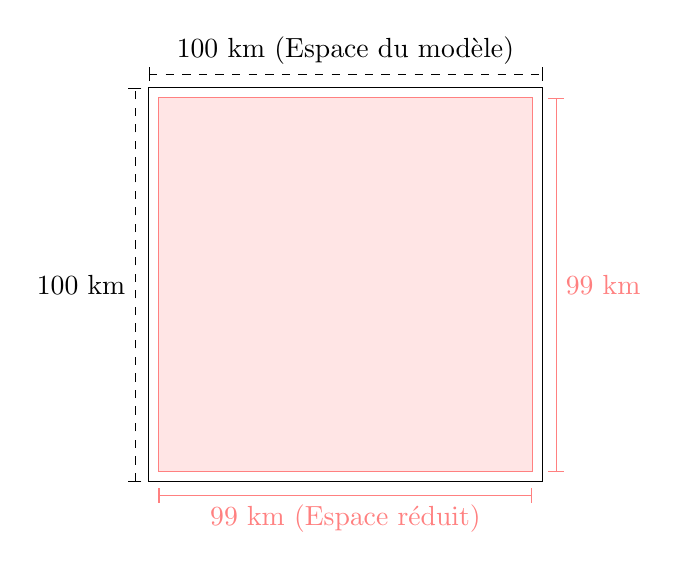
\begin{tikzpicture}[scale=.5]
	\draw[] (0,0) -- (0,10) -- (10,10) -- (10,0) -- cycle;
	\draw[|-|, very thin, dashed] (0, 10.35) -- node[above] {100 km (Espace du modèle)} (10, 10.35);
	\draw[|-|, very thin, dashed] (-0.35, 0) -- node[left] {100 km} (-0.35, 10);
	
	\draw[color=red!50, fill = red!10] (0.25, 0.25) -- (0.25, 9.75) -- (9.75, 9.75) -- (9.75, 0.25) -- cycle;
	\draw[|-|, red!50] (10.35, 9.75) -- node[right] {99 km} (10.35, 0.25);
	\draw[|-|, red!50] (0.25, -0.35) -- node[below] {99 km ({\color{red!50}Espace réduit})} (9.75, -0.35);
	\end{tikzpicture}
	\caption{Espace du modèle et espace \og utile\fg{}.}
\end{figure}
}

\subsubsection{Les agrégats de population}\marginnote{\hl{Développer et faire schémas}}[-20pt]

Un agrégat de population (village ou petite ville) est défini comme un ensemble d'au moins cinq foyers paysans espacés les uns des autres de moins de 100 m, cette distance étant un paramètre modifiable pour s'adapter à différents contextes régionaux.
Par convention, un village est défini comme un agrégat comportant de 5 à 29 foyers paysans ; une petite ville en comporte 30 ou plus.
Chaque agrégat de foyers paysans peut contenir une communauté.
Par défaut, aucun agrégat ne contient de communauté à sa création, mais à chaque pas de temps, il a une certaine probabilité (0,2 par défaut) d'en voir émerger une.
Une fois qu'un agrégat possède une communauté, il ne peut la perdre.
Quand un agrégat possède une communauté, on considère que l'ensemble des foyers paysans de cet agrégat font partie de ladite communauté.
Une communauté peut être plus ou moins puissante, influant fortement ou non sur la satisfaction des foyers paysans qui en font partie.
Cette puissance est variable d'une simulation à une autre mais identique pour toutes les communautés d'une simulation donnée.

\begin{figure}[H]
	\centering
	\marginnote{{\blueroman Nouveau schéma}}
	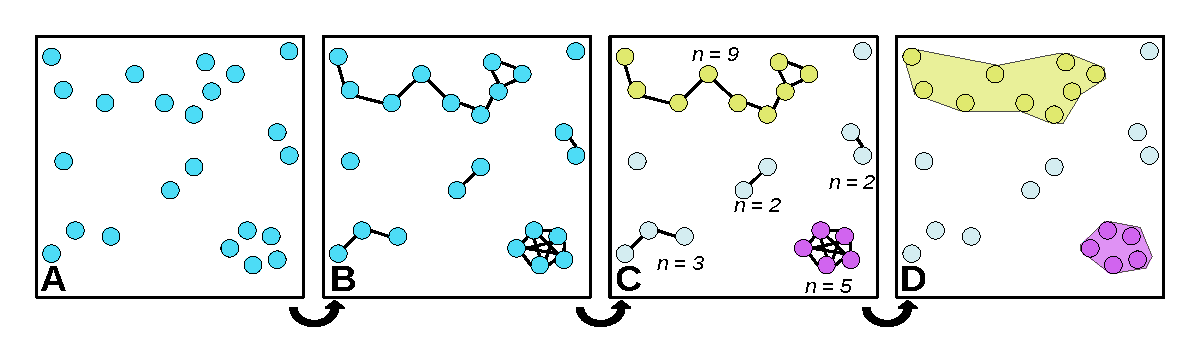
\includegraphics[width=1\linewidth]{src/identification_agregats.pdf}
	\caption{Méthode d'identification et de définition de forme des agrégats.\\On calcule un graphe composé de tous les foyers paysans situés à moins de $100$ mètres les uns des autres (\textbf{A}$\rightarrow$\textbf{B}) ; On compte le nombre de nœuds contenus dans chacune des \og grappes\fg{} identifiées (\textbf{B}$\rightarrow$\textbf{C}); On définit comme agrégats toutes les grappes composées d'au moins 5 foyers paysans (\textbf{C}$\rightarrow$\textbf{D}). L'agrégat est géométriquement défini comme l'enveloppe convexe des foyers paysans le composant (\textbf{D}).}
\end{figure}

{\blueroman A l'initialisation de SimFeodal, on crée plusieurs agrégats de populations dans l'espace restreint du modèle. Ces agrégats peuvent être des villages (10 foyers paysans) ou des agglomérations antiques (30 foyers paysans), dans les proportions identifiées thématiquement (\hl{tableau 3}).

\begin{table}[H]
\begin{center}
	\begin{tabular}{@{}|>{\centering\arraybackslash}m{.25\textwidth}|>{\centering\arraybackslash}p{.25\textwidth}|>{\centering\arraybackslash}p{.25\textwidth}|>{\centering\arraybackslash}p{.25\textwidth}|@{}}
		\hline
		\textbf{Nom} & \textbf{Variétés} & \textbf{Nombre par défaut en début de simulation} & \textbf{Objectif à atteindre en fin de simulation}  \\
		\hline
		\multirow{3}{*}[-2.5em]{Foyers Paysans} & Nombre & $4 000$ & $4000$ \\
		\cline{2-4}
		& Part de foyers paysans non mobiles (serfs, esclaves) & $20 \%$ & $20 \%$ \\
		\cline{2-4}
		& Part de foyers paysans dispersés & $95 \%$ environ & $20 \%$ \\
		\hline
		\multirow{3}{*}[.5em]{\makecell{Agrégats de\\population}} & Village & $20$ & $200$\\
		\cline{2-4}
		& Agglomération & 4 & 16\\
		\hline
	\end{tabular}  
\end{center}
\caption{Valeurs d'initialisation et d'objectifs des foyers paysans et agrégats. D'après (\hl{Peupler la terre, chap11})\\
	\todobox{Remettre les ndbp et la catégorisation estimation/données}\\}
\end{table}

Le mécanisme est le même pour chacun de ces agrégats : on commence par localiser aléatoirement un foyer paysan dans l'espace restreint du modèle. On crée ensuite un second foyer paysan à une distance inférieure à $100$ mètres du premier foyer paysan. On place ensuite, de la même manière, les foyers paysans suivants, en tirant aléatoirement l'un des foyers paysans déjà créés et en localisant le nouveau à une distance de moins de $100$ mètres.
On s'assure ainsi de constituer un agrégat de proche en proche.
}.


\subsubsection{Les foyers paysans}\marginnote{\hl{Développer !}}[-20pt]

Ne souhaitant pas représenter une évolution démographique au sujet de laquelle nous n'avons pas de certitude, nous partons du principe qu'en 800 comme en 1160, le nombre de foyers paysans est stable, arbitrairement fixé à 4 000.
Ces foyers correspondent à des groupes de quatre à cinq personnes, soit un espace peuplé de 16 000 à 20 000 habitants, c'est-à-dire une densité moyenne assez faible de l'ordre de 1,6 à 2 habitants par km2.
En 800, la plupart des foyers paysans sont dispersés de manière aléatoire dans l'espace modélisé (tableau 3).

\begin{figure}[H]
	\centering
	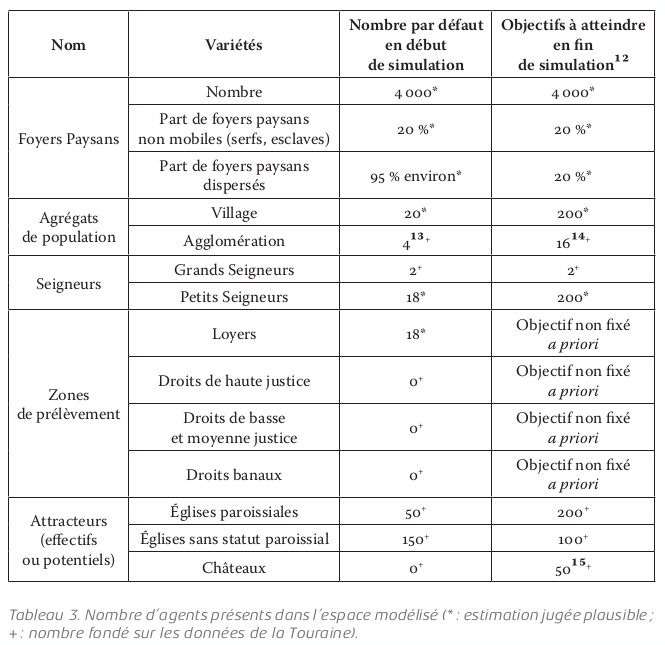
\includegraphics[width=1\linewidth]{src/Chapitre_TMD/Tab3.png}
	\caption*{
		\small
		12 : Ordre de grandeur.\\
		13 : Agglomérations secondaires d’origine antique. \\
		14 : En Indre-et-Loire (y compris les agglomérations d’origine antique).\\
		15 : Dont 10 à 15 gros châteaux.
}
\end{figure}

Au cours d'une simulation, nous considérons que la population se renouvelle partiellement, c'est-à-dire qu'à chaque pas de temps, une partie (5 \%, soit 200) des foyers paysans disparaît et le même nombre de foyers paysans apparaît.
Cela permet de représenter les sorties de système, soit que les foyers paysans aient changé de région, soit qu'ils n'aient pas eu de descendance. 
Les foyers paysans apparaissant en cours de simulation sont placés dans un agrégat choisi suivant un tirage aléatoire pondéré par le nombre de foyers paysans présents dans chaque agrégat.
Ce faisant, les foyers paysans concernés ont davantage de chances de se localiser dans un agrégat de grande taille plutôt que dans un agrégat de petite taille.

\subsubsection{Les seigneurs}\marginnote{\hl{Développer !}}[-20pt]

À l'initialisation du modèle, deux types de seigneurs coexistent : les premiers, que nous nommons « grands seigneurs », ont une portée d'action d'échelle supérieure, possèdent une puissance et des droits qui les placent loin devant les autres seigneurs en termes de pouvoir tant économique que militaire, ce qui fait d'eux des chefs de guerre.
Leur nombre est variable d'une région à l'autre, de même que leurs puissances relatives.
Dans l'exemple de la Touraine, on en décompte deux (les comtes d'Anjou et de Blois).
Ces seigneurs, contrairement aux seigneurs de moindre importance, sont en mesure d'intervenir sur tout le territoire, que ce soit pour y construire des châteaux ou y prélever des taxes et redevances.
Par opposition, les « petits seigneurs » sont plus nombreux (tableau 3), mais ont bien moins de pouvoir.
Ils prélèvent quelques taxes et redevances, en application de droits banaux le plus souvent, et possèdent quelques terres.
Leur portée d'action est locale : leur activité ne s'exerce qu'aux alentours de leur résidence, au sein de villages ou de petites villes.
De nouveaux petits seigneurs apparaissent peu à peu en cours de simulation et viennent s'ajouter à ceux initialement présents.
À leur création, ils ont uniquement des droits banaux, ou des droits de basse et moyenne justice qui s'appliquent à quelques foyers paysans dans leur voisinage.
Ces petits seigneurs apparaissant en cours de simulation n'obtiennent que rarement des droits fonciers : il s'agit d'une simplification du modèle au regard de la réalité historique.

\subsubsection{Les églises}

En 800, de nombreuses églises sont présentes (tableau 3), réparties de manière aléatoire dans l'espace du modèle. 
Certaines possèdent le droit de baptême et sont donc considérées comme églises paroissiales.
Les églises non paroissiales constituent une réserve d'édifices susceptibles de se voir doter de droits paroissiaux en cours de simulation.

\subsubsection{Attracteurs et pôles}

{\blueroman Ajouter texte et schéma décrivant l'identification des pôles depuis les attracteurs.}

\subsubsection{Initialisation technique de SimFeodal}

{\blueroman Ajouter schéma}

\subsection{Ordonnancement général des mécanismes}
{\blueroman
\begin{figure}[H]
	%% !TeX root = global_run.tex
%% !TeX encoding = UTF-8
%\documentclass[12pt, a4paper, oneside]{article}
%\usepackage{tikz}
%\usetikzlibrary{shapes,arrows}
%
%%%%<
%\usepackage{verbatim}
%\usepackage{makecell}
%
%\begin{document}

% Define block styles
\marginnote{{\blueroman Nouveau schéma}}
\tikzstyle{decision} = [diamond, draw, fill=blue!20, 
    text width=4.5em, text badly centered, node distance=3cm, inner sep=0pt]
\tikzstyle{block} = [rectangle, draw,
    minimum width=5em, align=center, rounded corners, minimum height=4em]

\tikzstyle{start} = [draw, circle, node distance=3cm,
    minimum height=2em, align=center]
\tikzstyle{line} = [draw, -latex']

\tikzstyle{legende} = [rectangle, draw,node distance=2.4cm,minimum size=2em,
    text width=5em, text centered, rounded corners, minimum height=2em]
\tikzstyle{fps} = [fill=green!60]
\tikzstyle{agregats} = [fill=blue!40]    
\tikzstyle{seigneurs} = [fill=yellow!20]
\tikzstyle{globals} = []
\tikzstyle{eglises} = [fill=red!40]
\tikzstyle{zps} = [fill=gray!20]
    
\begin{tikzpicture}[node distance = 3cm, auto]
    % Place nodes
    \node [start] (start) at (0,0) {Début\\du tour};
    \node [block, fps, right of=start] (renouvellement-fp) {Renouvellement\\des FP};
    
    
    \node [block, globals,right of=renouvellement-fp] (maj-globals) {MaJ des \\variables\\globales};
    \node [block, agregats, right of=maj-globals] (maj-agregats) {Détection\\des\\Agrégats};
    \node [block, seigneurs, right of=maj-agregats] (creation-seigneurs) {Création\\des nouveaux\\Seigneurs};
    \node [block, eglises,below of=creation-seigneurs] (maj-paroisses) {MaJ des\\contours des\\paroisses};
    \node [block, agregats, below of=maj-paroisses] (maj-poles) {Détection\\des\\Pôles};
    \node [block, globals, below of=maj-poles] (promo-chateaux) {Promotion\\des châteaux};
    
    \node [block, fps, below of=promo-chateaux] (deplacement-fp) {Déplacement\\des FP};
    \node [block, globals, left of=deplacement-fp] (maj-attrac) {MaJ\\attractivité\\châteaux et\\églises};
%    \node [block, eglises,left of=maj-chateaux] (maj-eglises) {MaJ eglises};
    \node [block, seigneurs, left of=maj-attrac] (maj-droits) {Gains de \\droits des\\seigneurs};
    \node [block, zps, left of=maj-droits] (maj-zp) {MaJ Zones de\\Prélèvement};
    \node [block, seigneurs, left of=maj-zp] (maj-dons) {Dons droits\\ et châteaux\\des Seigneurs};
    \node [block, seigneurs ,above of=maj-dons] (constructions-chateaux) {Constructions\\ des châteaux};
    \node [block, fps, above of=constructions-chateaux] (maj-satisfaction) {MaJ\\satisfactions\\des FP};
    
    \path[->, line]
    (renouvellement-fp) -- (maj-globals)
    (maj-globals) -- (maj-agregats)
    (maj-agregats) -- (creation-seigneurs)
    (creation-seigneurs) -- (maj-paroisses)
    (maj-paroisses) -- (maj-poles)
    (maj-poles) --(promo-chateaux)
    (promo-chateaux) -- (deplacement-fp)
    (deplacement-fp) -- (maj-attrac)
    (maj-attrac) -- (maj-droits)
    (maj-droits) -- (maj-zp)
    (maj-zp) -- (maj-dons)
    (maj-dons) -- (constructions-chateaux)
    (constructions-chateaux) -- (maj-satisfaction);
    \path [line, dotted]  (maj-satisfaction)-- (start);
    \path [line, dotted] (start) -- (renouvellement-fp);
    


\node [legende, agregats,below of=maj-dons, node distance = 3cm] (agregats) {Agrégats\\et Pôles};
\node [legende, fps, right of=agregats](fps) {Foyers\\Paysans};

\node [legende, seigneurs,right of=fps] (seigneurs) {Seigneurs};
\node [legende, eglises,right of=seigneurs] (eglises) {Églises};
\node [legende, zps,right of=eglises] (zps) {Zones de\\Prélèvement};
\node [legende, globals,right of=zps] (global) {Autre};

\end{tikzpicture}

%\end{document}
	
	\caption{test}
\end{figure}

Ajout du texte descriptif ici
}

\clearpage	
\section[Comportements des agents]{Description détaillée des comportements des agents}

Chaque type d'agents actifs dispose d'un degré d'initiative différent et poursuit des objectifs également différents.
Les agents « \textbf{foyers paysans} » se déplacent dans l'espace modélisé en fonction des modifications de leur environnement.
Localement, ces modifications consistent en la création de \textbf{paroisses}, la modification des ressorts paroissiaux, l'alourdissement des ponctions seigneuriales et l'apparition de \textbf{châteaux}.
Les modifications globales de l'environnement consistent, elles, en la naissance et le développement d'un climat de violence, ainsi qu'en l'accroissement des obligations religieuses.
Les agents « \textbf{seigneurs} » visent quant à eux à augmenter leur puissance en créant des \textbf{zones de prélèvement} et des \textbf{châteaux} et en développant leur réseau de fidèles.
Enfin les agents « \textbf{églises paroissiales} » se multiplient et modifient leur ressort dans le but de satisfaire le plus grand nombre de fidèles possible.
Les interactions entre les différents types d'agents se font uniquement via des entités spatiales : zones de prélèvement pour les interactions entre foyers paysans et seigneurs, ressorts paroissiaux pour les interactions entre foyers paysans et églises paroissiales.


\subsection{Foyers Paysans}

Les foyers paysans sont caractérisés par un ensemble de mesures de « satisfaction » qui les poussent à se déplacer lorsqu'elles sont trop faibles.
Ces déplacements s'effectuent selon des modalités particulières selon les situations, mais visent systématiquement à l'augmentation de la « satisfaction globale ».

\clearpage
\subsubsection{Satisfaction des foyers paysans}\marginnote{\hl{Développer !}}[-20pt]

La satisfaction globale d'un foyer paysan est une synthèse de trois mesures de satisfaction (matérielle, religieuse, et de protection face aux violences), dont on considère qu'elles ne se compensent pas mutuellement :
si l'une des mesures de satisfaction est faible, la satisfaction globale le sera également (cf. équation 1 du tableau 6).
Ces trois mesures sont les suivantes :
\begin{itemize}
	\item la satisfaction matérielle est une fonction des redevances dont doit s'acquitter le foyer paysan ($S_{redevances}$ – plus le foyer paysan doit s'acquitter de redevances, moins il est satisfait) et de son appartenance ou non à une communauté ($S_{communauté}$ – un foyer paysan est d'autant plus satisfait qu'il appartient à une communauté et que celle-ci est puissante).
	Le montant des redevances seigneuriales dont chaque foyer paysan doit s'acquitter ($redevances\_acquittées$) est la somme des droits des différents seigneurs dont dépend le foyer paysan (cf. équation 2 du tableau 6).
	
	\item la satisfaction religieuse correspond à la possibilité plus ou moins aisée d'accéder aux services liturgiques :
	se rendre à l'église et assurer le salut de son âme.
	Ceci est fonction de la distance à parcourir pour atteindre l'église paroissiale la plus proche ($distance\_eglise$).
	L'évaluation de cette distance varie au cours du temps et traduit une fréquentation accrue des foyers paysans (cf. équation 3 du tableau 6).
	
	\item la satisfaction en termes de protection est fonction de la distance entre le foyer paysan et le château le plus proche ($distance_{chateau}$) et du besoin de protection ressenti par le foyer paysan ($besoin\_protection$).
	Celui-ci apparaît à partir de 960 et correspond à la naissance et au développement d'une conflictualité entre seigneurs locaux résultant de la perte d'influence du pouvoir central (cf. équation 4 du tableau 6).
\end{itemize}

\begin{figure}[H]
	\centering
	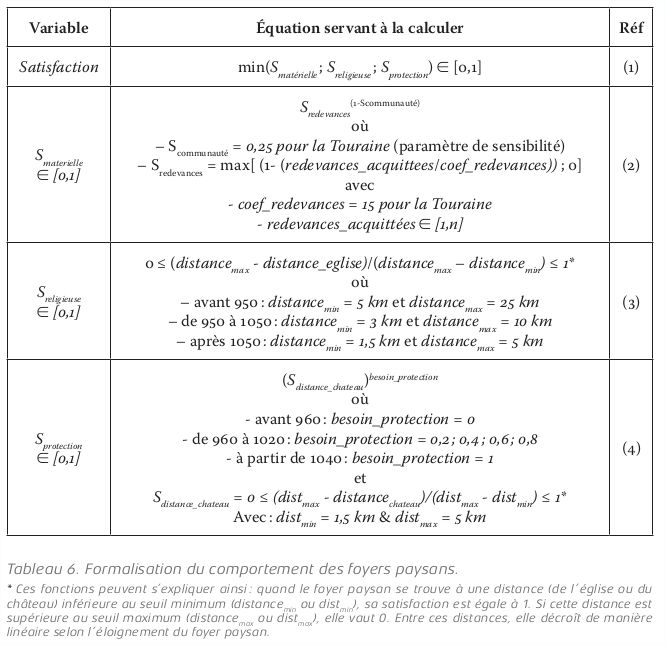
\includegraphics[width=1\linewidth]{src/Chapitre_TMD/Tab6.png}
	\marginnote{\hl{Modifier et développer tableau}}[-50pt]
\end{figure}

\clearpage
\subsubsection{Déplacement des foyers paysans}\marginnote{\hl{Développer !}}[-20pt]

\begin{figure}[H]
	%% !TeX root = FP_deplacement.tex
%% !TeX encoding = UTF-8
%\documentclass[10pt, a4paper, oneside]{article}
%\usepackage{tikz}
%\usetikzlibrary{shapes,arrows}
%
%%%%<
%\usepackage{verbatim}
%\usepackage{makecell}
%
%\begin{document}
	
	% Define block styles
	\tikzstyle{start} = [draw, circle,
	minimum height=3em, align=center, fill = green!40]
	\tikzstyle{end} = [draw, circle,
	minimum height=2em, align=center, fill = red!40]
	\tikzstyle{decision} = [diamond, draw, fill=yellow!20, 
	text width=3em, align=center, inner sep=0pt]
	\tikzstyle{block} = [rectangle, draw,
	minimum width=3em, align=center, rounded corners, minimum height=3em]
	
	
	\tikzstyle{line} = [draw, -latex']

	
	\begin{tikzpicture}[node distance = 4cm, auto]
	% Nodes
	\node [start] (start) {Début du\\déplacement};
	\node [decision, below of=start] (mobile) {FP mobile ?};
	\node [end,left of=mobile] (fixe) {Pas de\\déplacement};
	\node [decision, below of=mobile] (tirage-satis) {$n_1\sim\mathcal{U}(0,1)$*};
	\node [decision, below of=tirage-satis] (tirage-rnd) {$n_2\sim\mathcal{U}(0,1)$*};
	\node [block, left of=tirage-rnd] (local) {Déplacement\\local};
	\node [block, right of=tirage-rnd] (lointain) {Déplacement\\lointain};
	\node [decision, left of=local] (pole-local) {Pôle\\à\\proximité ?};
	\node [block, below of=pole-local] (lotterie-locale) {Lotterie\\pondérée :\\
	Attractivité des\\ Pôles locaux};
	\node  [end, right of=lotterie-locale] (fin-local) {Déplacement\\dans le\\pôle vainqueur};
	
	\node [block, below of=lointain] (lotterie-agregats) {Lotterie\\pondérée :\\
		Attractivité\\des\\ Agrégats};
	\node  [end, left of=lotterie-agregats] (fin-lointain) {Déplacement\\dans \\l'agrégat\\vainqueur};
	
	% Paths
	\path [->, line] (start) -- (mobile);
	\path [->, line] (local) -- (pole-local);
	\path [->, line] (lotterie-locale) -- (fin-local);
	\path [->, line] (lointain) -- (lotterie-agregats);
	\path [->, line] 	(lotterie-agregats) -- (fin-lointain);
	
	 \draw [->, dotted](mobile) -- (fixe) node [midway, above, sloped] (TextNode) {Non};
	 \draw [->, dotted](mobile) -- (tirage-satis) node [midway, right] (TextNode) {Oui};
	 \draw [->, dotted] (tirage-satis) -| (fixe) node [near start, below] (TextNode) {$n_1 < (1 - Satis)$};
	 \draw [->, dotted](tirage-satis) -- (tirage-rnd) node [midway, right] (TextNode) {$n_1 \ge (1 - Satis)$};
	 \draw [->, dotted](tirage-rnd) -- (lointain) node [midway, below] (TextNode) {$n_2 \leq 0.2$};
	 \draw [->, dotted](tirage-rnd) -- (local) node [midway, below] (TextNode) {$n_2 > 0.2$};
	 \draw [->, dotted] (pole-local) |- (fixe) node [near start, left] (TextNode) {Non};
	 \draw [->, dotted] (pole-local) -- (lotterie-locale) node [midway, left] (TextNode) {Oui};
	\end{tikzpicture}
	
	\footnotetext[1]{Tirage aléatoire}
%\end{document}

	\caption{Diagramme d'activité des mécanismes de déplacement des foyers paysans.\\
		* : Tirage aléatoire d'une variable ($n_1$ et $n_2$) dans une distribution uniforme contenue entre $0$ et $1$.}
\end{figure}


\begin{figure}[H]
	\centering
	\marginnote{{\blueroman Reprise d'un schéma non publié dans le chapitre de Peupler la Terre}}
	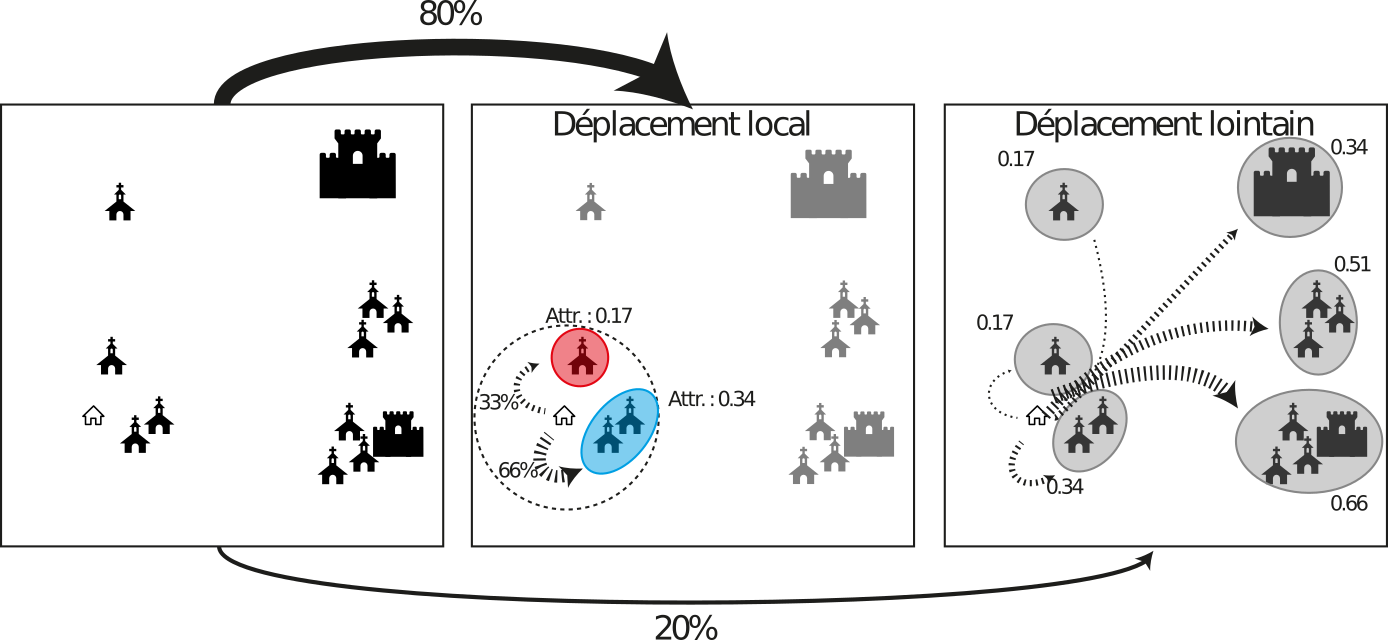
\includegraphics[width=1\linewidth]{img/Deplacement.png}
	\caption{Déplacement locaux et déplacements lointains.}
	\marginnote{\hl{Adapter pour pôles vs agrégats}}[-50pt]
\end{figure}

À chaque pas de temps, chaque foyer paysan a une certaine probabilité de se déplacer.
Ce déplacement vise à augmenter sa satisfaction en se rapprochant d'un pôle d'attraction.

La plupart des déplacements se font localement :
\begin{itemize}
	\item le foyer paysan identifie le pôle le plus attractif localement, c'est-à-dire dans un rayon de 2,5 km (une demi-heure de marche) de sa localisation actuelle ;
	\item si la probabilité de déplacement local ($p[deplacement\_local]$\footnote{
		$p(deplacement\_local) = max[(\text{Attractivité du pôle le plus attractif localement} – Satisfaction) ; 0].$	
	}) se réalise, un tirage aléatoire pondéré par les attractivités respectives des pôles de son environnement va déterminer où le foyer paysan va s'implanter.
	Un pôle d'attraction est constitué d'un ou plusieurs attracteurs proches les uns des autres (à moins de 200 m) (cf. tableau 7).
	La valeur d'attraction d'un pôle correspond à la somme des attractivités des attracteurs le composant, pour traduire la différenciation importante de l'attraction des pôles qu'entraîne le nombre d'attracteurs présents \autocite[tableau 13, p. 96]{zadora-rio_paroisses_2008}.
	\item si la probabilité de déplacement local ne se réalise pas, le foyer paysan a une (faible) probabilité d'effectuer un déplacement lointain ($p[deplacement\_lointain]$\footnote{
		$p(deplacement\_lointain) = 0,2 × (1 – Satisfaction)$.
	}).
\end{itemize}

\begin{figure}[H]
	\centering
	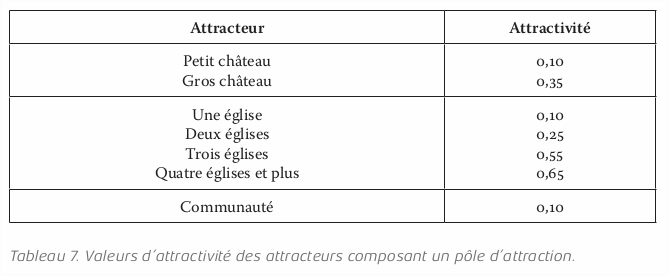
\includegraphics[width=1\linewidth]{src/Chapitre_TMD/Tab7.png}
	\marginnote{\hl{Modifier et développer tableau}}[-50pt]
\end{figure}

\clearpage
\subsection{Seigneurs}

\subsubsection{Construction de châteaux}

Au fur et à mesure de la simulation, des châteaux sont créés, au départ par les grands seigneurs uniquement, puis par tout seigneur suffisamment puissant.
Un grand seigneur peut créer un ou plusieurs châteaux, soit au sein d'un agrégat qui n'en contient pas encore, soit en dehors des agrégats existants, à une distance minimale des châteaux antérieurs.
La probabilité pour un grand seigneur de créer un ou des châteaux croît au fur et à mesure de l'augmentation de sa puissance (tableau 4).
La création d'un château implique nécessairement celle d'une zone de prélèvement de loyers associée :
tous les foyers paysans situés à l'intérieur de cette zone de prélèvement s'acquittent d'un loyer au seigneur détenteur de la zone.
Dans le modèle, la création d'un château implique également la création de zones de prélèvement de droits banaux et/ou de droits de basse et moyenne justice de même rayon que la zone de prélèvement de loyers, sous condition que le seigneur soit déjà par ailleurs détenteur de ces droits.
Quand un petit seigneur devient suffisamment puissant, il peut aussi créer un château (tableau 4) et devient alors seigneur châtelain.
À ce titre, il prélève les loyers et les droits banaux et de basse et moyenne justice associés au château.
Ce château est forcément localisé à proximité du seigneur, c'est-à-dire dans l'agrégat de population le plus proche de lui, si celui-ci ne possède pas déjà un château.
À partir de 940, certains châteaux gagnent énormément en attractivité et deviennent de gros châteaux (figure 2).
Historiquement, leur promotion est liée à la création de marchés, de prieurés et de bourgs.
Cependant, ces éléments n'étant pas représentés dans le modèle, chaque château a simplement une probabilité de devenir un gros château.
Cette probabilité est beaucoup plus forte si le château est situé dans un village déjà doté d'une église (tableau 4).


\begin{figure}[H]
	\centering
	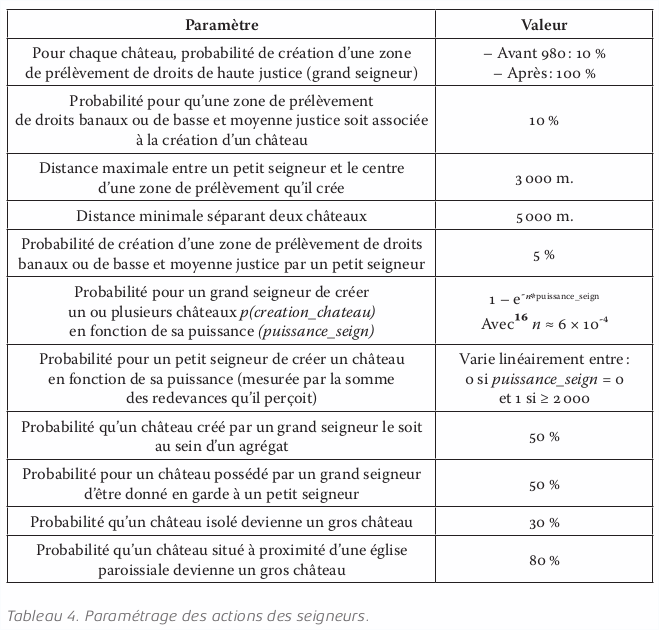
\includegraphics[width=1\linewidth]{src/Chapitre_TMD/Tab4.png}
			\caption*{
		\small
		16 : Cela permet d’avoir une probabilité fortement croissante pour les valeurs moyennes, puis bornée rapidement : avec cette valeur de $n$, on obtient 0 pour une puissance de 0, environ 0,5 pour une puissance de 1000, et cela converge lentement vers 1 au-delà.
	}
	\marginnote{\hl{Modifier et développer tableau}}[-50pt]
\end{figure}

\clearpage
\subsubsection{Acquisition et prélèvement de droits seigneuriaux}

Le prélèvement des redevances et droits seigneuriaux se fait au sein d'une zone de prélèvement, dont les attributs sont le détenteur (seigneur qui l'a créée), le rayon et le taux de prélèvement (tableau 5).
Dans les cas où les zones de prélèvement sont liées à un château, leur rayon dépend de la puissance du propriétaire du château comparée au minimum et maximum de puissance des autres seigneurs au moment de la création de la zone.

\begin{figure}[H]
	\centering
	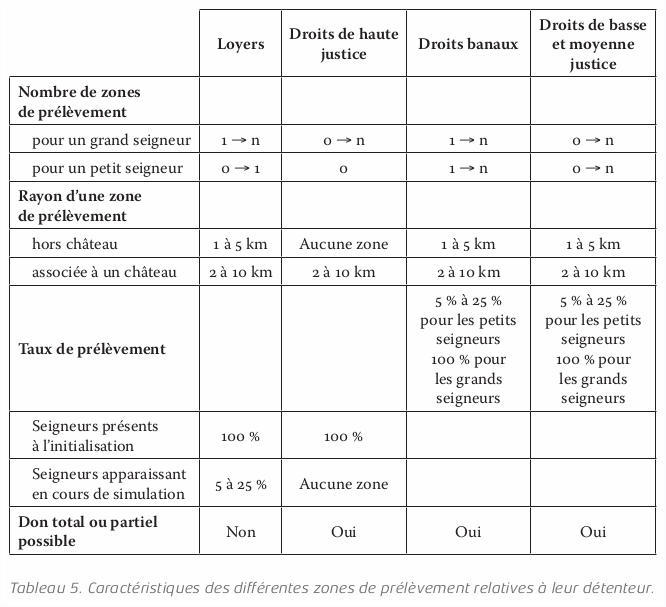
\includegraphics[width=1\linewidth]{src/Chapitre_TMD/Tab5.png}
	\marginnote{\hl{Modifier et développer tableau}}[-50pt]
\end{figure}



La totalité des foyers paysans payent un loyer.
Ceux situés dans une zone de prélèvement de loyer s'en acquittent au seigneur possédant la zone (figure 3).
Quand les foyers paysans ne sont pas situés dans une telle zone ou que celle-ci n'a pas un taux de prélèvement de 100 \%, ce sont les grands seigneurs qui prélèvent ce loyer.
Au fur et à mesure de la création de châteaux et des zones associées, le prélèvement des loyers est de plus en plus associé aux châteaux.
Les prélèvements associés aux châteaux représentent non seulement les redevances payées par chaque foyer paysan en échange de la protection du châtelain, mais aussi les ponctions sur les récoltes et autres troubles occasionnés par les conflits armés entre seigneurs autour du château.

\begin{figure}[H]
	\centering
	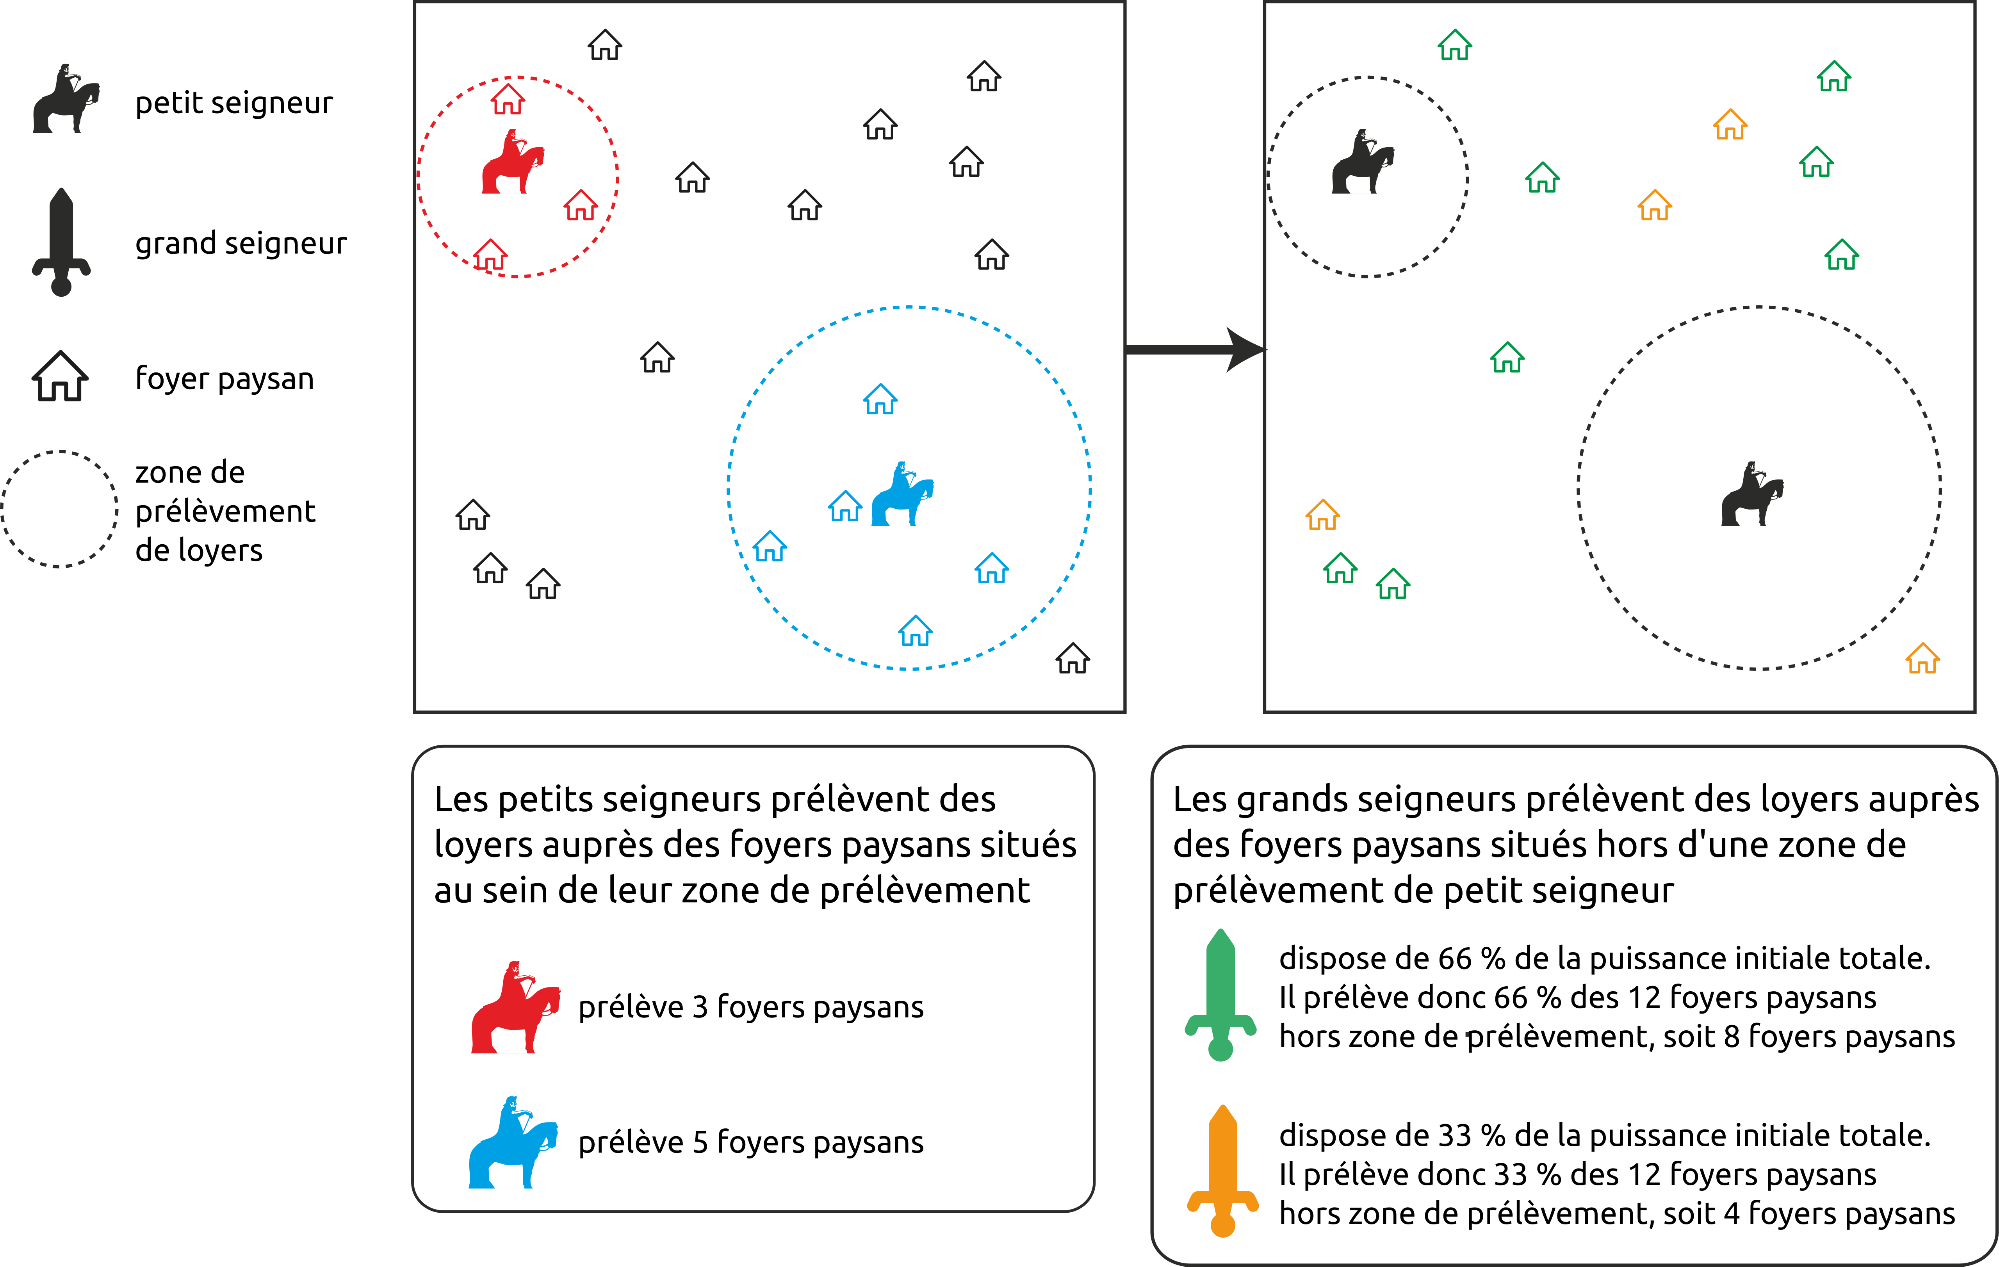
\includegraphics[width=1\linewidth]{src/Chapitre_TMD/Fig3}
	\caption{Prélèvements des loyers par les seigneurs.}
	\label{fig:fig3}
\end{figure}

\paragraph{Grands Seigneurs}
Les grands seigneurs acquièrent les droits de haute justice au cours d'une simulation, entre 900 et 1000 pour la Touraine (figure 2).
Ce faisant, en l'année de simulation 1000, chaque grand seigneur dispose d'une zone de prélèvement de ces droits autour de chacun de ses châteaux. 
Ces zones de prélèvement représentent une source de richesse importante.
Dans le modèle, la totalité des foyers paysans situés dans une telle zone s'acquittent des droits de haute justice au seigneur détenteur de la zone (tableau 5).
La création d'une zone de prélèvement de droits de haute justice entraîne la création de deux autres zones de prélèvement de même rayon et de même détenteur correspondant au prélèvement de droits banaux et de droits de basse et moyenne justice.
La totalité des foyers paysans situés dans ces zones de prélèvement s'acquittent de ces droits au seigneur détenteur.
Entre 900 et 980, les grands seigneurs qui n'ont pas encore de zone de prélèvement de droits de haute justice peuvent acquérir des droits banaux ou de basse et moyenne justice selon une probabilité de 0,1 à chaque pas de simulation.
Quand ils acquièrent ces droits, ils créent une zone de prélèvement associée autour de tous leurs châteaux.
Finalement, en 1000, les grands seigneurs prélèvent chacun les loyers et les différents types de droits (basse, moyenne et haute justice, droits banaux) autour de tous leurs châteaux.

\paragraph{Petits Seigneurs}
Au cours de la simulation, les petits seigneurs acquièrent des droits banaux et/ou de basse et moyenne justice sur les foyers paysans qui leur sont assujettis.
On le modélise par la probabilité pour un petit seigneur, à chaque pas de simulation, de créer une zone de prélèvement de taille modeste dans son voisinage (tableau 5).
Ces droits peuvent s'accumuler (figure 4).

\begin{figure}[!h]
	\centering
	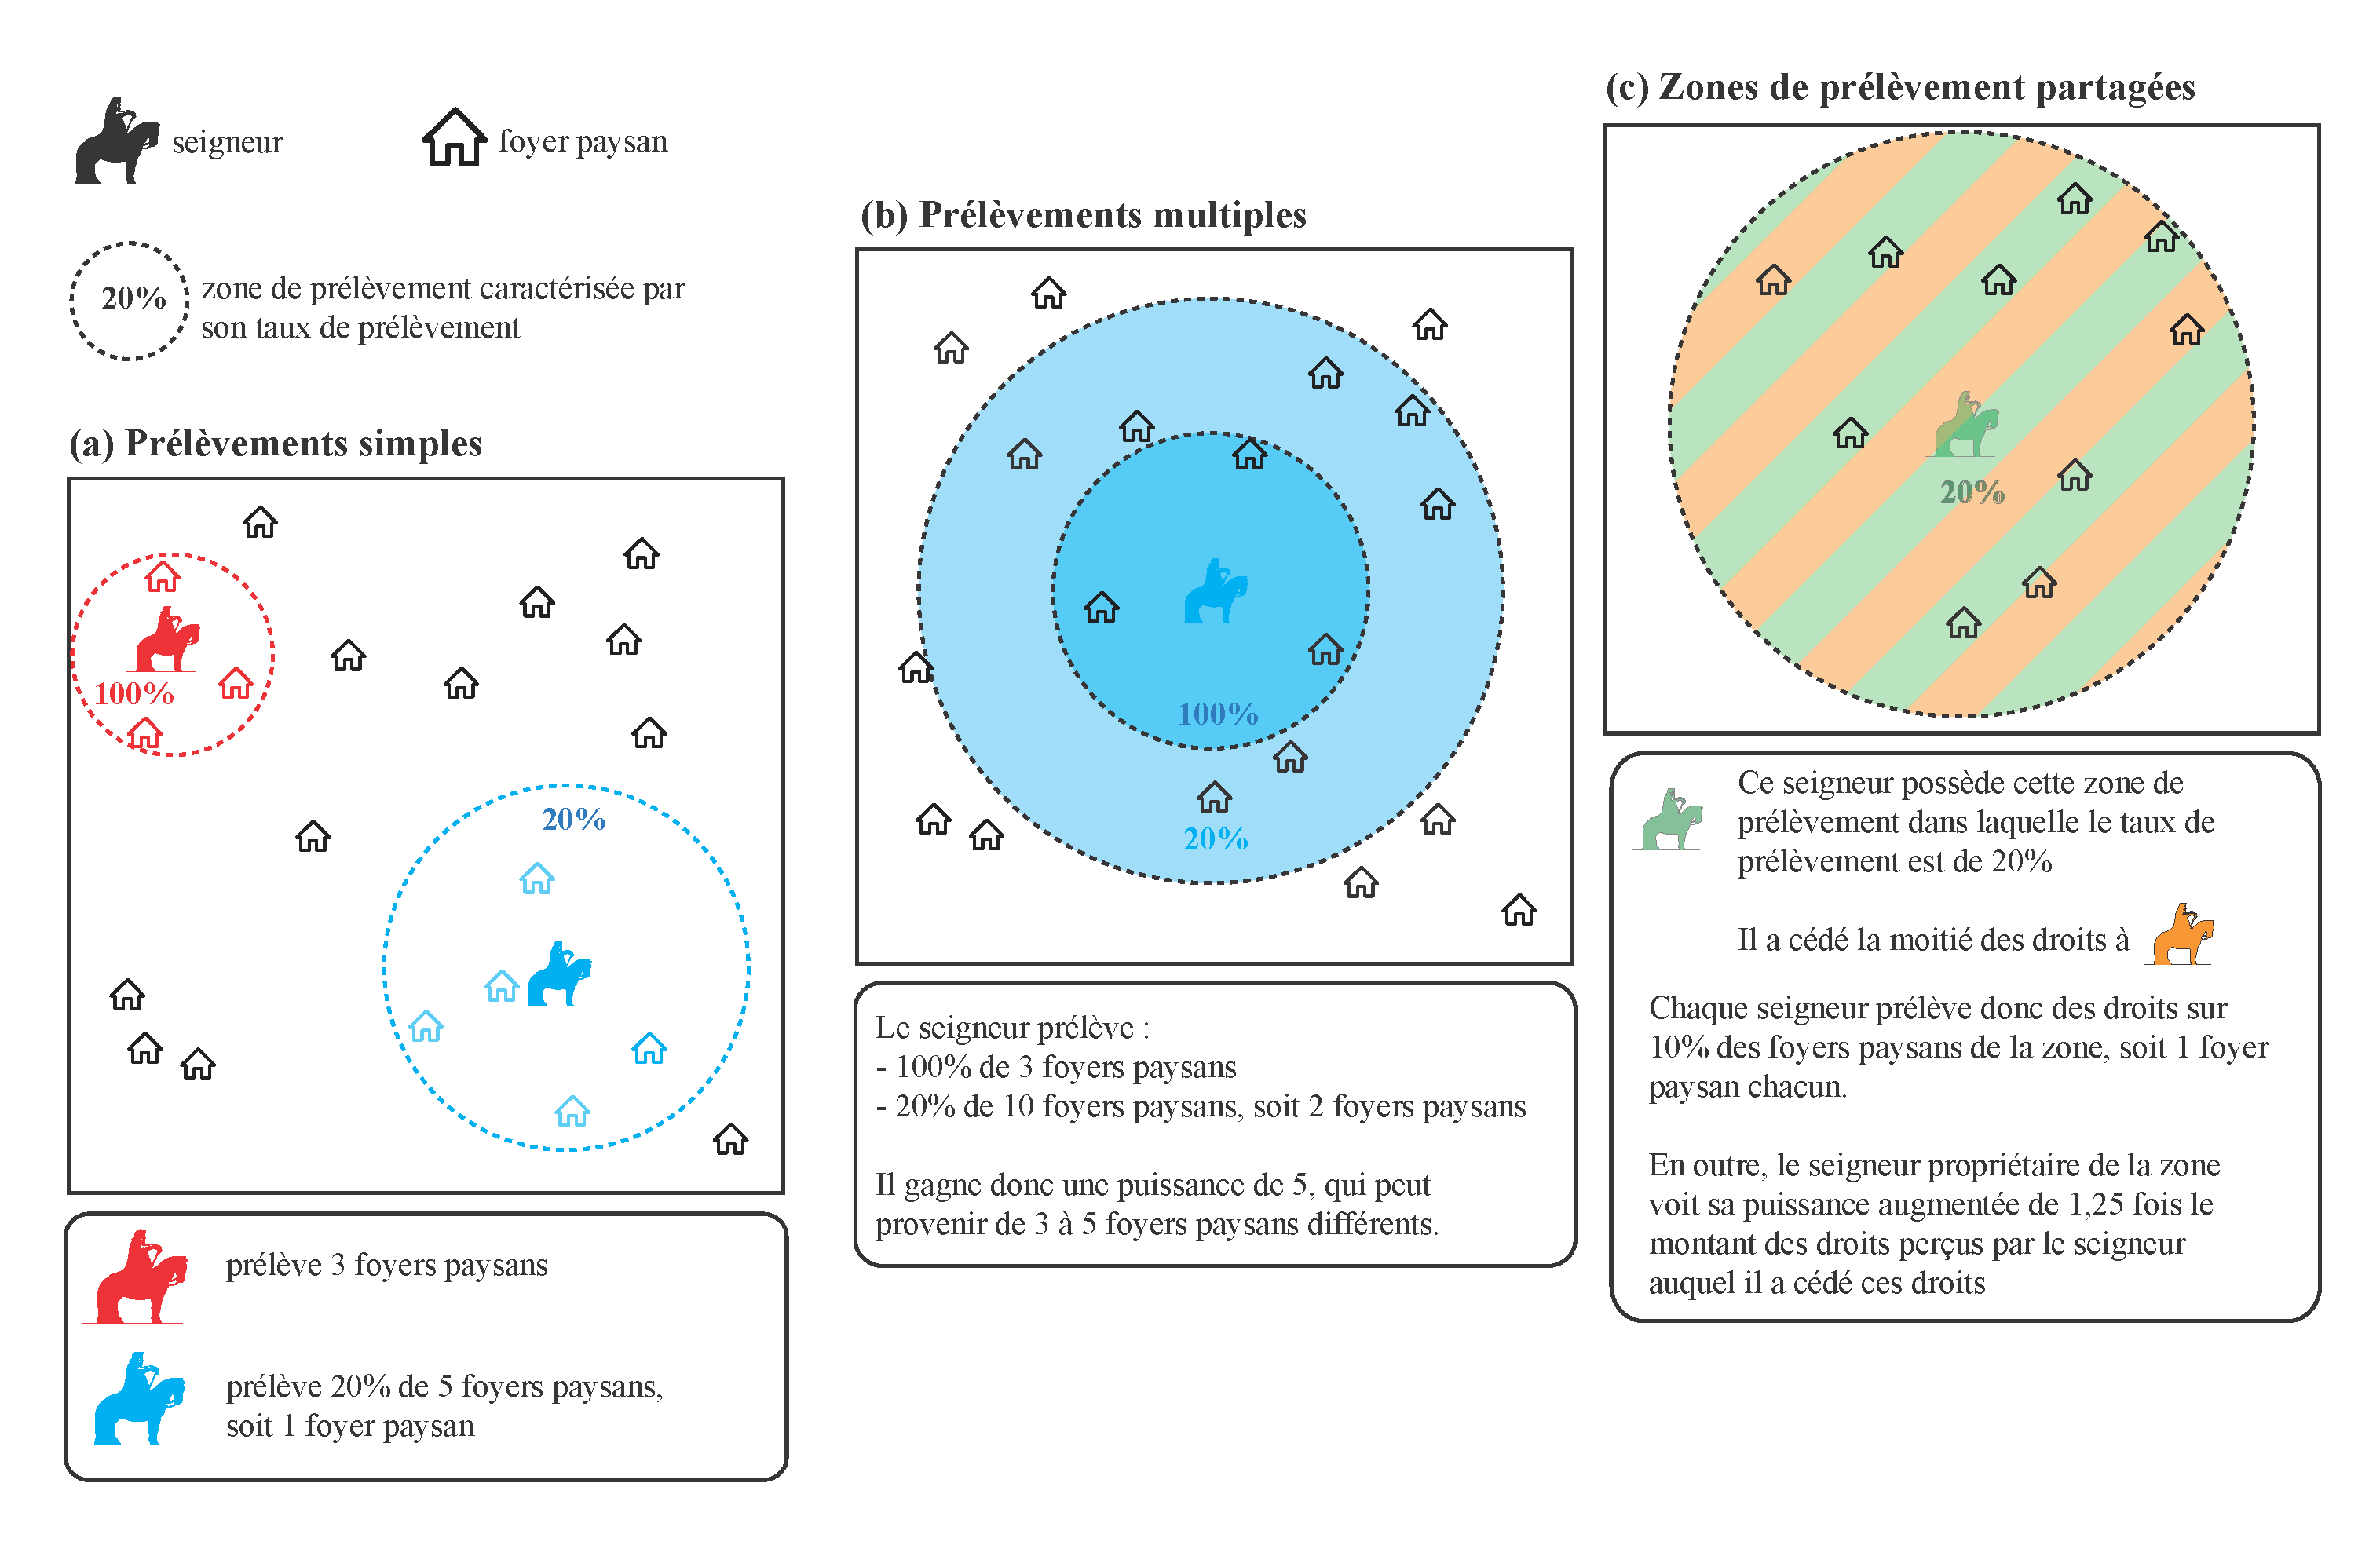
\includegraphics[width=1\linewidth]{src/Chapitre_TMD/Fig4}
	\caption{Superposition des droits prélevés par les seigneurs sur les foyers paysans : différents cas de figure.}
	\label{fig:fig4}
\end{figure}

\subsubsection{Cession de droits seigneuriaux}

À partir de 880 environ, les relations de vassalité entre les seigneurs s'institutionnalisent (figure 2).
Dans la relation féodale, le seigneur protège son vassal et le vassal contribue à la puissance armée du seigneur.
Les seigneurs cèdent une partie de leurs droits à d'autres seigneurs moins puissants en échange de leur fidélité.
\paragraph{Grands Seigneurs}
Un grand seigneur peut céder des droits à un petit seigneur qui n'est pas déjà le vassal d'un autre grand seigneur :
dans ce cas, il crée une nouvelle zone de prélèvement.
Celle-ci est localisée dans un agrégat, pris au hasard parmi tous.
Elle a une chance sur trois d'être de « droits banaux », « droits de haute justice » ou « droits de basse et moyenne justice » et son rayon est défini aléatoirement dans un intervalle donné (même principe que pour les petits seigneurs s'arrogeant de nouveaux droits).
Le taux de prélèvement (i. e. la part de foyers paysans prélevés dans la zone) est fixé à 100 \%.
Le grand seigneur demeure le détenteur de la zone tandis que le petit seigneur en perçoit les redevances :
pour chaque foyer paysan assujetti à cette redevance, le grand seigneur (détenteur) percevra 1,25 point (droits de haute justice) ou 0,35 point (droits banaux ou de basse et moyenne justice), et le petit seigneur à qui elle a été cédée percevra respectivement 1 ou 0,25 point.
Le petit seigneur récipiendaire du don devient vassal du grand seigneur.
\paragraph{Petits Seigneurs}
Les petits seigneurs qui détiennent des zones de prélèvement peuvent aussi céder tout ou partie des droits qu'ils possèdent dessus :
pour chaque zone de prélèvement qu'ils détiennent, ils ont une probabilité (33 \% à chaque pas de simulation) d'en céder une partie, par pas de 5 \%, à un autre petit seigneur éloigné de moins de 3 km.
L'attribution des redevances des foyers paysans aux petits seigneurs se fait de la même manière que pour les grands seigneurs.
Ainsi, chaque zone de prélèvement a une liste de récipiendaires associés à un taux de perception des redevances de la zone.
La somme de ces taux vaut 100 \% quand toute la zone de prélèvement a été cédée par le seigneur détenteur à un ou plusieurs seigneurs récipiendaires.

\paragraph{Don de châteaux en gardiennage}
À partir de 960, quand un grand seigneur possède plusieurs châteaux, on considère qu'il peut en donner certains à garder à un seigneur de son entourage (figure 2).
Par convention, on considère dans le modèle que le seigneur gardien d'un château perçoit toutes les redevances des zones de prélèvement associées au
château.
Sur la zone de prélèvement des revenus fonciers, il perçoit la totalité des droits.
Les autres types de droit (droits de justice, droits banaux...) sont gagnés progressivement (1/3 à chaque pas de temps).

\subsubsection{Puissance des seigneurs}

La puissance d'un seigneur est calculée par le modèle à chaque pas de simulation.
Elle se présente sous deux formes :
\begin{itemize}
\item \textbf{Puissance issue des redevances perçues}: elle représente la richesse et l'influence d'un seigneur.
C'est au travers de cet indicateur qu'est estimée la possibilité pour un seigneur de construire un château (variable intitulée $puissance\_seign$ dans le tableau 4).
Chaque seigneur acquiert de la puissance par le prélèvement de redevances auprès des foyers paysans dans les zones de prélèvement qu'il possède.
Ces redevances perçues peuvent l'être directement ou indirectement, via le don de tout ou partie d'une zone de prélèvement.
Comme chaque foyer paysan est amené à s'acquitter de plusieurs droits différents, chacun sera donc pris en compte de multiples fois dans le calcul de cette puissance.
Les foyers paysans ne rétribuant pas, au sens propre, les seigneurs suzerains de leurs seigneurs locaux, cet indicateur de puissance représente aussi une forme quantifiable d'influence ou de visibilité, puisqu'on considère qu'un don de château ou de droits profite directement à celui qui l'effectue.

\item \textbf{Puissance armée}: elle correspond au nombre de foyers paysans qui sont assujettis à un seigneur, quels que soient les droits concernés et que ce soit à travers une zone de prélèvement dont il est détenteur ou récipiendaire.
Elle n'intervient pas dans la dynamique du modèle mais peut être étudiée en sortie de simulation.
La puissance armée correspondant au cas où un seigneur est donateur d'une partie de ses zones de prélèvements permet de représenter la capacité de mobilisation militaire d'un seigneur influent, qui pourra demander des troupes à ses vassaux.
\end{itemize}


\clearpage
\subsection{Les églises}\marginnote{\hl{Développer}}[-30pt]

\subsubsection{Définition des paroisses}

{\blueroman Ajouter texte et schéma pour décrire la définition des paroisses en zones de Voronoï}

\begin{figure}[!h]
	\centering
	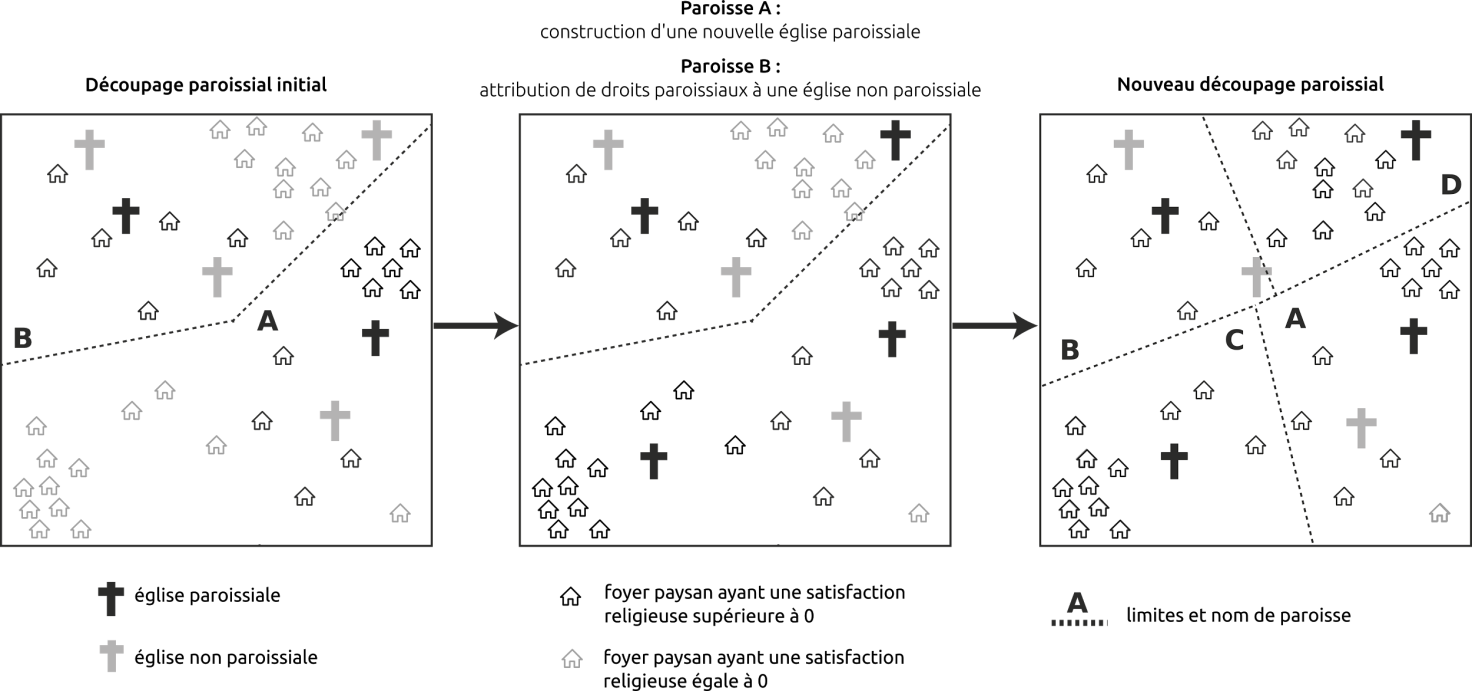
\includegraphics[width=1\linewidth]{src/Chapitre_TMD/Fig5}
	\caption{Création de nouvelles paroisses et modification de paroisses existantes.}
\label{fig:fig5}
\end{figure}

{\blueroman Subdiviser schéma + ajout création paroisses dans subsubsec suivante pour ajouter mécanisme création paroisses dans agrégats}

\clearpage
\subsubsection{Création et promotion d'églises paroissiales}
De nouvelles églises, construites par les seigneurs laïques ou les communautés religieuses, viennent s'ajouter à celles qui existaient avant 800 (tableau 3), et leur rôle d'attracteur se renforce avec la mise en place, au cours de la transition, du système paroissial sur lequel les évêques exercent un contrôle croissant.
Les églises paroissiales, qui focalisent les pratiques cultuelles et sociales, deviennent des lieux centraux à l'échelle locale.
Elles déterminent des aires d'attraction dont la territorialisation s'est progressivement affirmée.
Les polygones de Thiessen\footnote{
Partition complète de l’espace en fonction de la densité de points.
} permettent de découper l'espace du modèle de telle sorte que chaque église paroissiale soit au centre d'une zone définie comme étant son ressort paroissial (figure 5).
Les églises non paroissiales sont susceptibles de se voir doter de droits paroissiaux en cours de simulation, selon une probabilité fixée à 0,5.
En outre, de nouvelles églises paroissiales sont construites à partir de 960, dans ou à proximité d'agrégats de foyers paysans, selon une probabilité égale à :
$$P(creation\_eglise\_agregat) = \frac{1}{seuil\_creation\_eglise} × \frac{nb\_FPagregat}{nb\_paroissesagregat}$$
Le terme $nb\_FPagregat$ correspond au nombre de foyers paysans dans
l'agrégat et le terme $nb\_paroissesagregat$ au nombre de ressorts paroissiaux inclus dans, ou intersectant, l'agrégat entouré d'une zone tampon de 200 m de large.
Le paramètre $seuil\_creation\_eglise$ est fixé à 100 foyers paysans.
Une fois ces nouvelles églises paroissiales créées, l'espace du modèle fait l'objet d'un nouveau découpage afin d'actualiser les contours des ressorts paroissiaux.
Au sein de chaque ressort paroissial, on calcule la satisfaction religieuse de chaque foyer paysan.
Si au moins dix foyers paysans ont une satisfaction religieuse égale à zéro, une nouvelle paroisse est créée\footnote{
	\todobox{Modifier et développer largement pour rendre plus compréhensible en incorporant dans le corps du texte}\\
Selon les règles suivantes, dépendant du nombre d’églises non paroissiales dans le ressort :
\begin{itemize}
	\item supérieur à 3, la plus éloignée d’entre elles devient paroissiale ;
	\item entre 1 et 3, l’une d’entre elles (au hasard) devient paroissiale ;
	\item égal à 0, s’il en existe à moins de 2 km alentour, une devient paroissiale (au hasard) ;
\end{itemize}
}.

L'espace du modèle fait alors l'objet d'un nouveau découpage afin d'actualiser les contours des ressorts paroissiaux et de tenir compte des nouvelles paroisses lors du calcul de la satisfaction religieuse des foyers paysans.


\section{Quelques résultats de simulation}\marginnote{\hl{Supprimer partie}}[-30pt]


\toChange{Les premières simulations effectuées}{Conserver et déplacer ce paragraphe.} ont eu pour objectif de vérifier que le modèle fournit des résultats plausibles pour la Touraine modélisée.
Le modèle comporte plusieurs tirages probabilistes (par exemple, pour déterminer si un foyer paysan effectue un déplacement local ou lointain, ou pour déterminer si un château devient un gros château, ou encore pour déterminer si une nouvelle église paroissiale va être créée ou non au sein d'un agrégat de foyers paysans).
Par conséquent, pour un même jeu de valeurs de variables et de paramètres, les résultats fournis par le modèle sont susceptibles de varier d'une simulation à une autre.
Plusieurs réplications d'une même simulation sont donc nécessaires pour analyser les résultats (vingt réplications ici).

\begin{figure}[H]
	\centering
	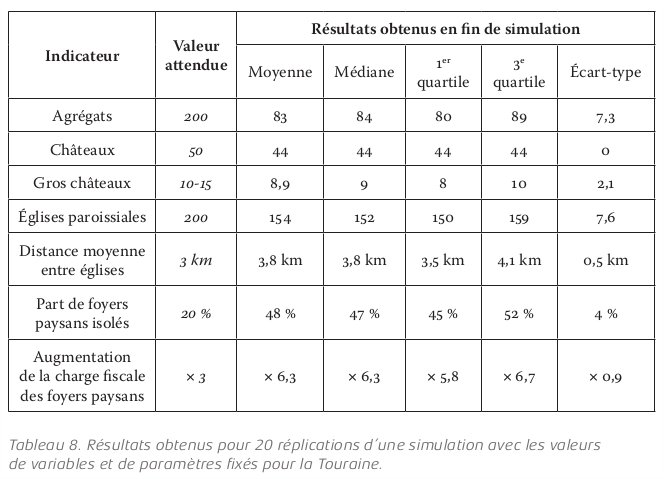
\includegraphics[width=1\linewidth]{src/Chapitre_TMD/Tab8.png}
	\marginnote{\hl{Modifier et développer tableau}}[-50pt]
\end{figure}

\begin{figure}[!h]
	\centering
	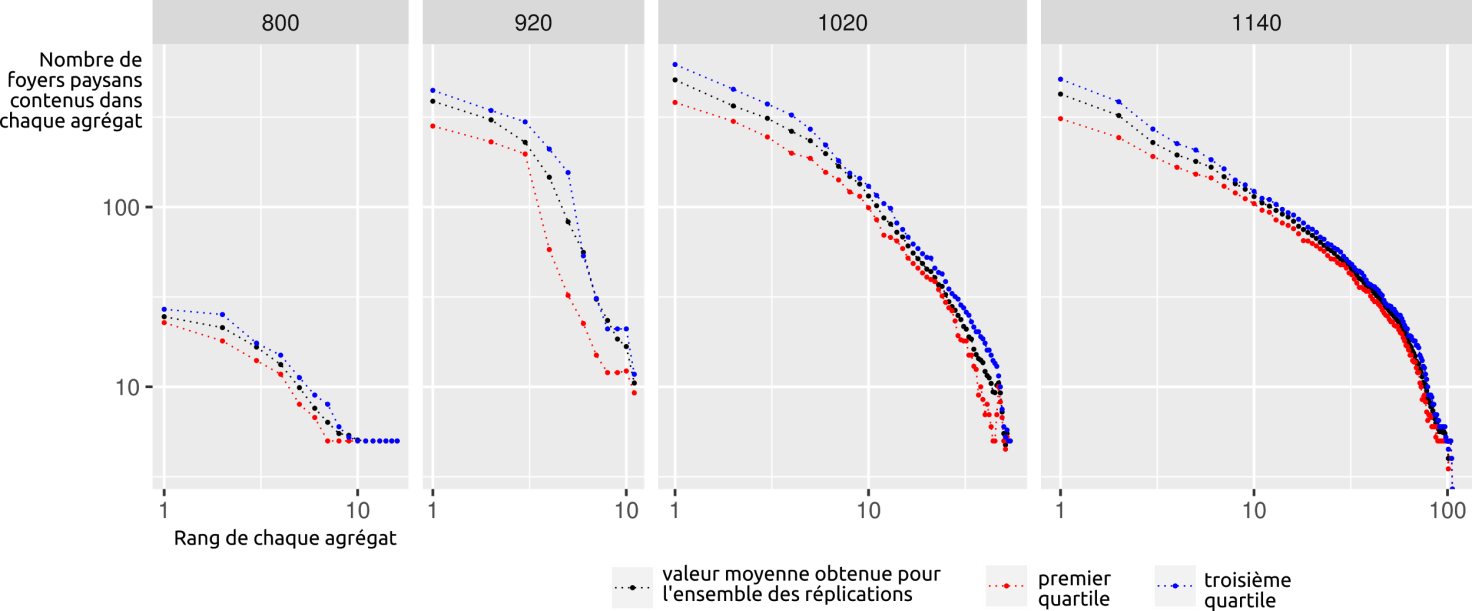
\includegraphics[width=1\linewidth]{src/Chapitre_TMD/Fig6}
	\caption{
		\todobox{Modifier/enlever}\\
		Distributions rang-taille des agrégats obtenues pour vingt réplications d'une simulation avec les valeurs de variables et de paramètres fixés pour la Touraine.}
	\label{fig:fig6}
\end{figure}

Le tableau 8 montre que les résultats obtenus sont souvent assez proches des ordres de grandeur attendus.
Les variables pour lesquelles les résultats du modèle diffèrent des résultats attendus sont le nombre d'agrégats de foyers paysans, trop faible, et la proportion de foyers paysans isolés (c'est-à-dire localisés hors d'un village ou d'une ville), trop élevée.
Sur ces aspects, le modèle simule un processus de polarisation insuffisamment puissant mais qui pourrait être intensifié en modifiant certaines valeurs de variables et de paramètres.
En revanche, le modèle reproduit bien le processus de hiérarchisation du système de peuplement (figure 6).
Le nombre d'agrégats de foyers paysans croît en effet tout au long de la période de simulation.
La taille des agrégats change aussi au fil du temps : au départ compris entre 5 et 40 foyers paysans environ en 800, les plus gros agrégats rassemblent presque 200 foyers paysans en 920, et encore un peu plus à partir de 1020, étant entendu que le nombre d'habitants est constant tout au long de la simulation.

\begin{figure}[!h]
	\centering
	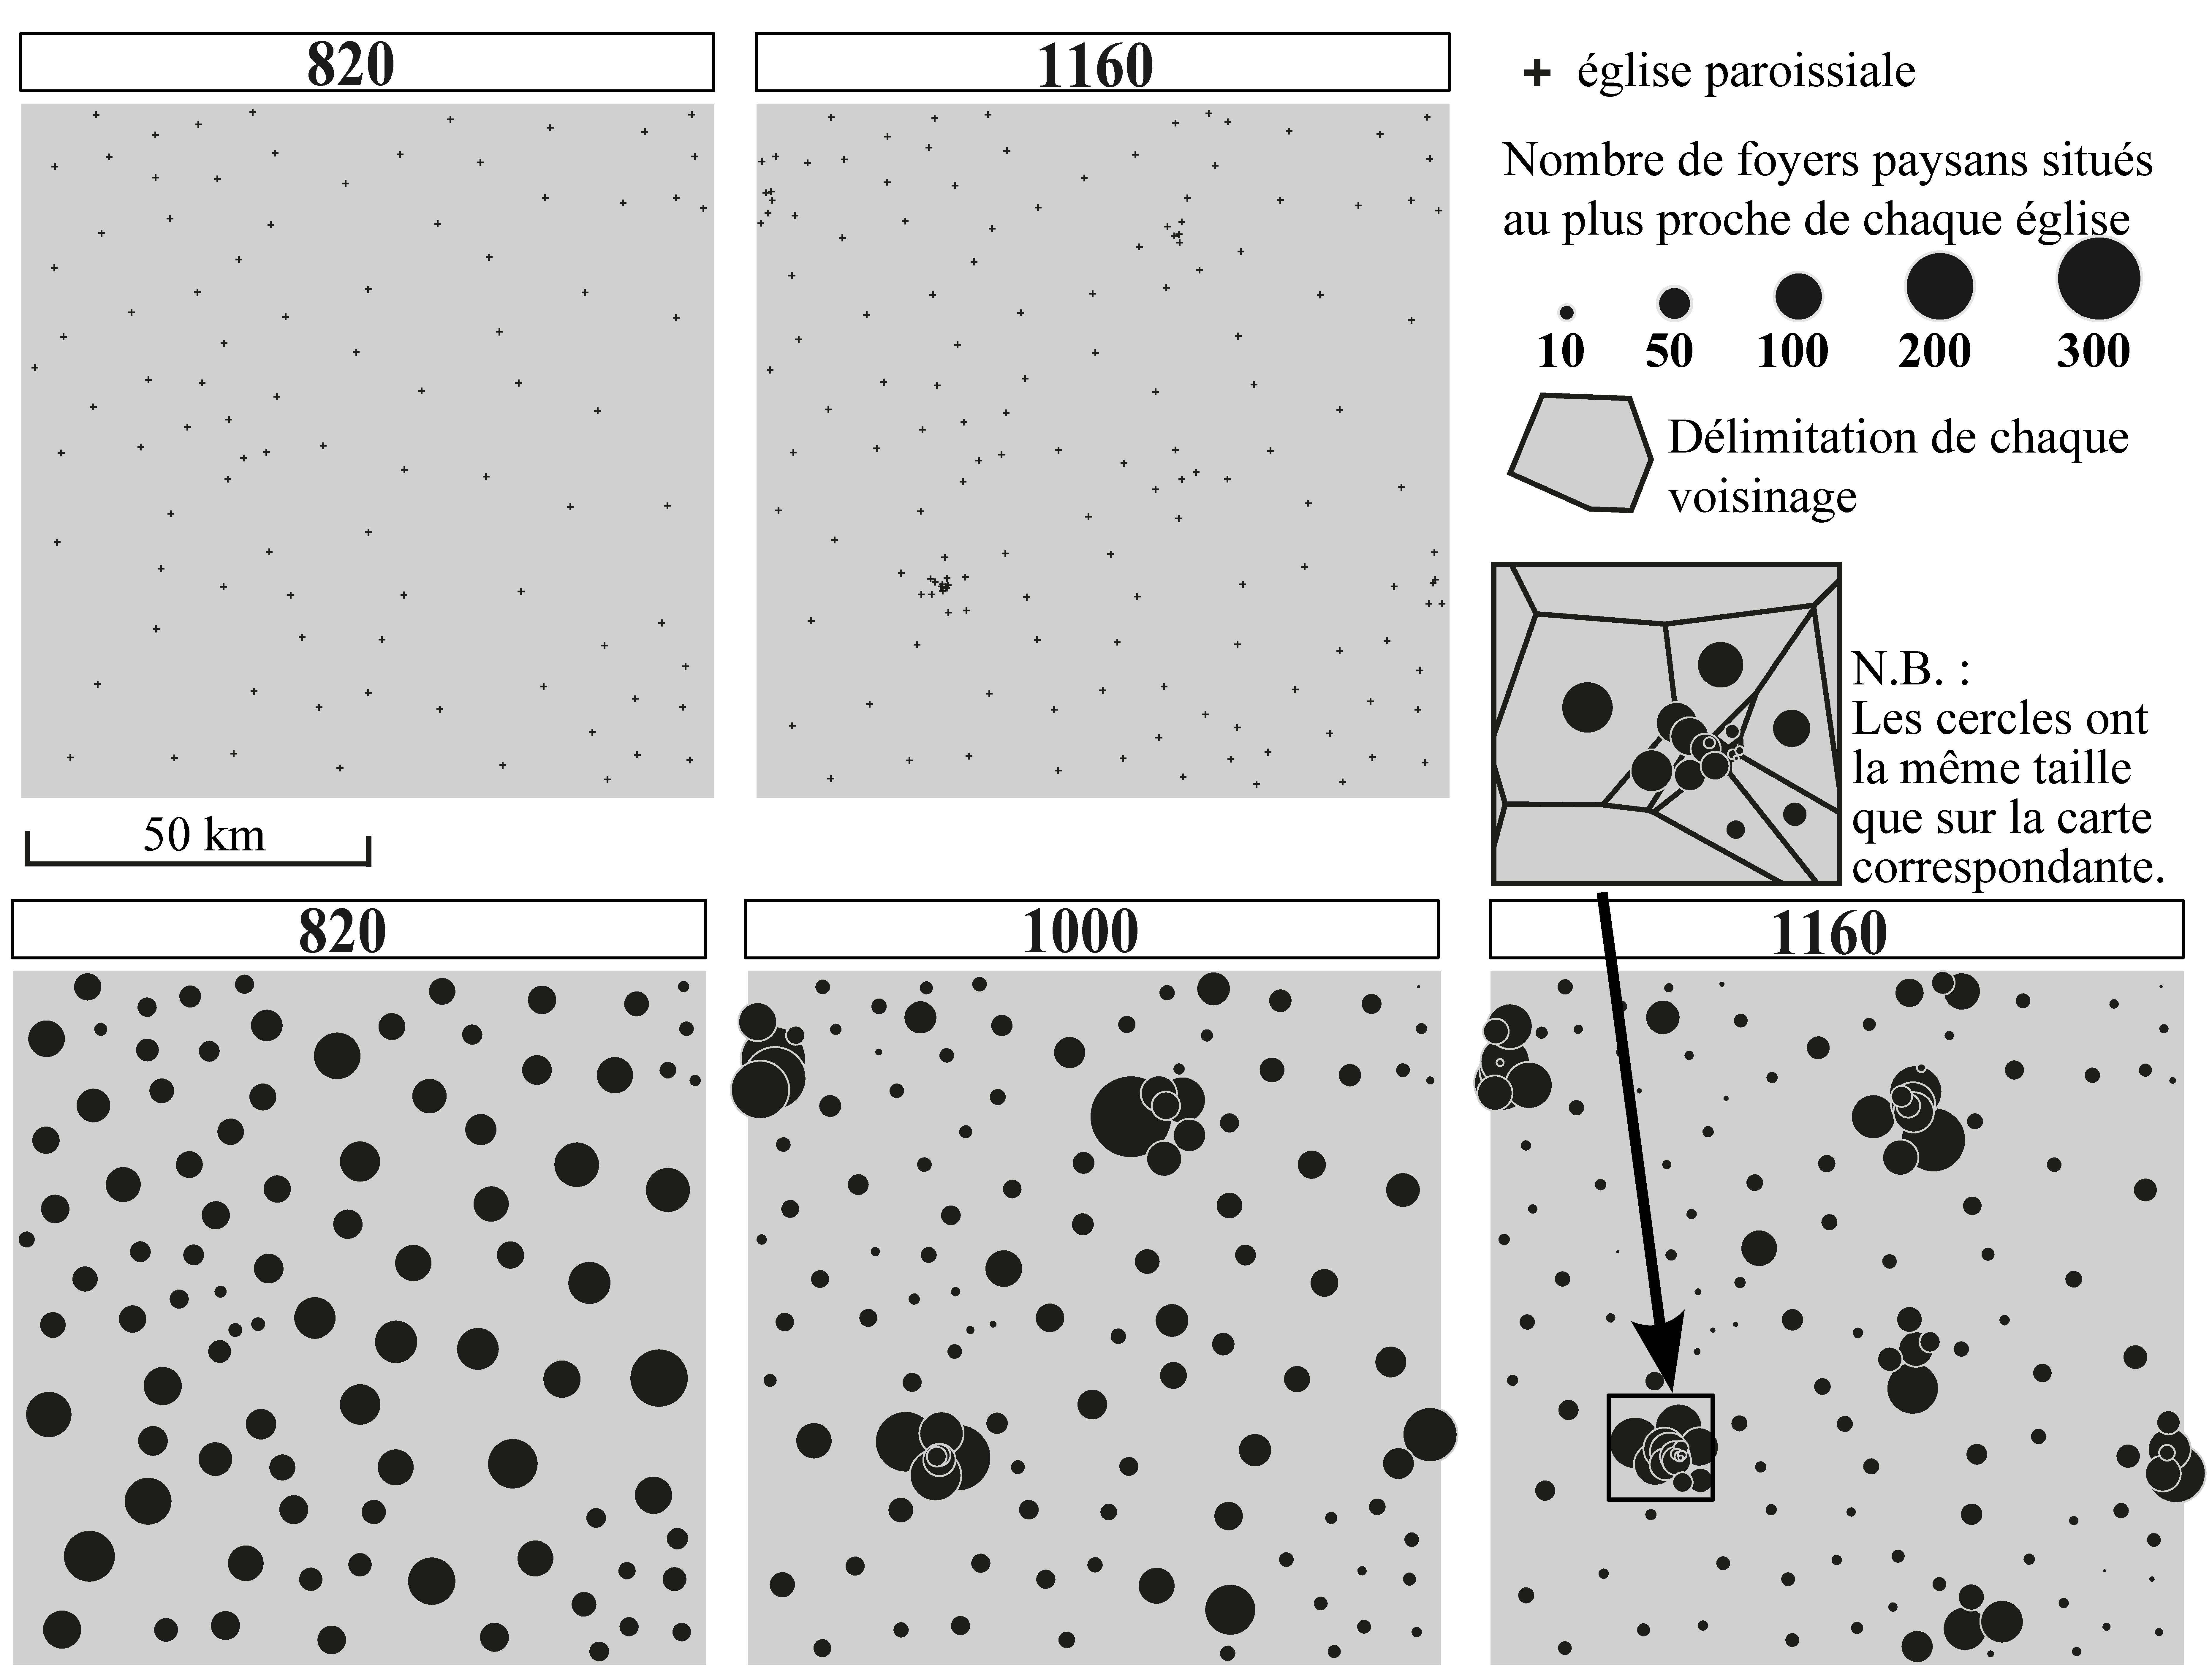
\includegraphics[width=1\linewidth]{src/Chapitre_TMD/Fig7}
	\caption{Églises paroissiales créées par simulation et nombre de foyers paysans dans leur voisinage (défini au moyen d’une tessellation de Voronoï).
	Exemple d’une réplication parmi les vingt simulées.
	Les églises paroissiales existent avant le début de la période, mais les territoires (ou les ressorts) paroissiaux émergent au cours de la transition.
	Ces voisinages représentent donc les paroisses en fin de période, et une construction du modèle auparavant.}
	\label{fig:fig7}
\end{figure}

Cette hiérarchisation ainsi que le processus de polarisation sont visibles dans l'espace du modèle (figure 7\footnote{
Dans chaque ressort paroissial, et ici pour chacun des cercles proportionnels, les foyers paysans peuvent être soit dispersés (surtout en début de période de simulation), soit concentrés dans des agrégats de population (en fin de période).
}).
On constate que la population, dispersée en début de simulation, tend vers une forte concentration autour de quelques pôles majeurs en fin de période.
Cette évolution est accompagnée par le développement et la structuration du réseau des églises paroissiales.

\section*{Conclusion}

\toChange{L'étude qui est présentée ici}{Conserver et déplacer ce paragraphe} est un cas d'application de modélisation et de simulation dans un contexte interdisciplinaire.
Nous avons cherché à dégager des faits stylisés qui conservent un niveau de complexité acceptable et accepté par les experts du domaine.
Toute démarche de modélisation suppose une simplification, mais il ne s'agissait pas pour nous d'aboutir à une vision simpliste des processus considérés.
Pour ce faire, nous sommes passés graduellement d'une description littéraire des phénomènes à leur représentation sous des formes plus abstraites, pour finalement parvenir à la définition d'entités (objets) implémentées dans un modèle multi-agents : SimFeodal.
La phase suivante du travail est dans l'ajustement des paramètres.

Nous espérons que ce modèle apporte un éclairage renouvelé sur la période et les phénomènes considérés.
Cependant, cet apport du modèle n'est pas encore attesté ; il doit maintenant être soumis à la communauté des chercheurs du domaine.
Ceci est notre objectif à court terme.
